\documentclass[11pt]{article}

\usepackage[a4paper]{geometry}
\geometry{left=2.0cm,right=2.0cm,top=2.5cm,bottom=2.5cm}

\usepackage{ctex} % 支持中文的LaTeX宏包
\usepackage{amsmath,amsfonts,graphicx,amssymb,bm,amsthm,mathrsfs,mathtools,breqn} % 数学公式和符号的宏包集合
\usepackage{siunitx} % 国际单位制宏包
\usepackage{algorithm,algorithmicx} % 算法和伪代码的宏包
\usepackage[noend]{algpseudocode} % 算法和伪代码的宏包
\usepackage{fancyhdr} % 自定义页眉页脚的宏包
\usepackage[framemethod=TikZ]{mdframed} % 创建带边框的框架的宏包
\usepackage{fontspec} % 字体设置的宏包
\usepackage{adjustbox} % 调整盒子大小的宏包
\usepackage{fontsize} % 设置字体大小的宏包
\usepackage{tikz} % 绘制图形和使用颜色的宏包
\usetikzlibrary{arrows.meta,positioning} % TikZ箭头库和定位库
\usepackage{float} % 支持[H]浮动体位置参数
\usepackage{multicol} % 多栏排版的宏包
\usepackage{multirow} % 表格中合并单元格的宏包
\usepackage{pdfpages} % 插入PDF文件的宏包
\RequirePackage{listings} % 在文档中插入源代码的宏包
\usepackage{wrapfig} % 文字绕排图片的宏包
\usepackage{bigstrut,rotating} % 支持在表格中使用特殊命令的宏包
\usepackage{booktabs} % 创建美观的表格的宏包
\usepackage{circuitikz} % 绘制电路图的宏包
\usepackage{pgfplots} % 绘图宏包
\pgfplotsset{compat=1.18}
\usepackage{hyperref} % 创建超链接的宏包
\usepackage{subcaption} % 支持子图标题的宏包
\usepackage[inline]{enumitem} % 自定义列表格式的宏包，支持行内列表

\definecolor{dkgreen}{rgb}{0,0.6,0}
\definecolor{gray}{rgb}{0.5,0.5,0.5}
\definecolor{mauve}{rgb}{0.58,0,0.82}
\lstset{
  frame=tb,
  aboveskip=3mm,
  belowskip=3mm,
  showstringspaces=false,
  columns=flexible,
  framerule=1pt,
  rulecolor=\color{gray!35},
  backgroundcolor=\color{gray!5},
  basicstyle={\small\ttfamily},
  numbers=none,
  numberstyle=\tiny\color{gray},
  keywordstyle=\color{blue},
  commentstyle=\color{dkgreen},
  stringstyle=\color{mauve},
  breaklines=true,
  breakatwhitespace=true,
  tabsize=3,
}


\usepackage[capitalize]{cleveref}
\Crefname{section}{Section}{Sections}
\Crefname{table}{Table}{Tables}
\crefname{table}{Table.}{Tabs.}

\setmainfont{Palatino Linotype}
\setCJKmainfont{SimSun}[BoldFont=SimHei, ItalicFont=KaiTi]
\setCJKsansfont{SimHei}
\setCJKmonofont{FangSong}
\punctstyle{kaiming}
% 偏好的几个字体, 可以根据需要自行加入字体ttf文件并调用

% Restore standard emphasis to avoid requiring an undefined environment (kaishu).
% The original redefinition used an environment `kaishu` which is not defined
% in a default ctex setup and causes compilation errors. Use \textit for
% emphasis which works across engines.
\renewcommand{\emph}[1]{\textit{#1}}

%改这里可以修改实验报告表头的信息
\newcommand{\experiName}{RLC电路的谐振现象}
\newcommand{\supervisor}{李国强}
\newcommand{\name}{邓思豪}
\newcommand{\studentNum}{2023K8009909008}
\newcommand{\class}{3}
\newcommand{\group}{01}
\newcommand{\seat}{5}
\newcommand{\dateYear}{2025}
\newcommand{\dateMonth}{11}
\newcommand{\dateDay}{12}
\newcommand{\room}{西实204}
\newcommand{\others}{$\square$}


\begin{document}



\begin{center}
    \LARGE \bf 《\, 基\, 础\, 物\, 理\, 实\, 验\, 》\, 实\, 验\, 报\, 告
\end{center}

\begin{center}
    \noindent \emph{实验名称}\underline{\makebox[25em][c]{\experiName}}
    \emph{指导教师}\underline{\makebox[8em][c]{\supervisor}}\\
    \emph{姓名}\underline{\makebox[6em][c]{\name}} 
    % 如果名字比较长, 可以修改box的长度"6em"
    \emph{学号}\underline{\makebox[10em][c]{\studentNum}}
    \emph{分班分组及座号} \underline{\makebox[5em][c]{\class \ -\ \group \ -\ \seat }\emph{号}} （\emph{例}:\, 1\,-\,04\,-\,5\emph{号}）\\
    \emph{实验日期} \underline{\makebox[3em][c]{\dateYear}}\emph{年}
    \underline{\makebox[2em][c]{\dateMonth}}\emph{月}
    \underline{\makebox[2em][c]{\dateDay}}\emph{日}
    \emph{实验地点}\underline{{\makebox[6em][c]\room}}
    \emph{调课/补课} \underline{\makebox[3em][c]{\others\ 是}}
    \emph{成绩评定} \underline{\hspace{5em}}
    {\noindent}
    \rule[8pt]{17cm}{0.2em}
\end{center}

\section{实验目的}
本实验通过理论分析与实验观测相结合的方式，聚焦RLC电路的核心特性，明确以下目标：
\begin{enumerate}
    \item 深入研究RLC串联电路的谐振现象
        掌握RLC串联电路在正弦激励下谐振状态的物理本质，明确谐振时电路阻抗（最小且呈纯阻性）、回路电流及各元件端电压的分布规律；掌握谐振频率的理论推导公式与实验测量方法，理解谐振过程中电感与电容间的能量交换机制及外部电源的能量供给特点。
    
    \item 系统掌握RLC电路的频率特性
        全面理解RLC电路的幅频特性（电路响应幅值随激励频率变化的规律）与相频特性（响应与激励信号的相位差随频率变化的规律）；明确幅频特性中品质因数（$Q$值）对谐振峰尖锐程度的调控作用，掌握实验测绘频率特性曲线的方法，理解频率特性在电路选频、滤波功能中的应用逻辑。
    
    \item 观测暂态过程并理解阻尼振动规律
        利用数字存储示波器的波形存储与分析功能，观测RLC串联电路在阶跃激励下的暂态响应；分析欠阻尼、临界阻尼、过阻尼三种条件下电路的暂态衰减（或振动）规律，理解阻尼系数对暂态过程的影响，建立电路“稳态特性-暂态响应”的关联认知。
\end{enumerate}

\section{实验仪器与用具}
本实验采用的仪器设备涵盖电路核心元件、信号激励源、观测与测量工具，各设备的功能与参数适配实验对电路调控、信号输出、特性观测的需求，具体配置及作用如下：
\begin{enumerate}
    \item 标准电感：提供标称值稳定的感性元件，作为RLC电路的感性支路核心单元，其低损耗特性可降低谐振过程的能量衰减误差，保障电路参数的可重复性。
    
    \item 标准电容：提供标称值稳定的容性元件，作为RLC电路的容性支路核心单元，具备低介质损耗特性，可减少谐振频率与电压分布的测量偏差。
    
    \item 100Ω标准电阻：高精度固定阻值电阻，既是RLC串联电路的基础电阻部件，也可配合数字多用表完成电路参数的校准与验证。
    
    \item 电阻箱：步进式可调电阻装置，用于灵活调控RLC电路的等效电阻，实现欠阻尼、临界阻尼、过阻尼等不同暂态条件的切换，同时适配幅频特性的阻尼调控需求。
    
    \item 电感箱：可调式电感装置，支持对RLC电路感性参数的精准配置，便于验证不同电感值下的谐振频率、暂态阻尼规律。
    
    \item 电容箱：可调式电容装置，支持对RLC电路容性参数的精准配置，与电感箱配合可实现不同谐振频率的电路调试，适配幅频特性的参数变量需求。
    
    \item 函数发生器：多波形信号源，可输出频率可调的正弦波（用于稳态幅频/相频特性测试）与方波（阶跃激励，用于暂态过程观测），为电路提供可控激励信号。
    
    \item 数字存储示波器：具备波形存储、幅值量化、相位差分析功能的观测设备，用于捕捉RLC电路的电压波形、测绘频率特性曲线，以及记录暂态阻尼振动的动态过程。
    
    \item 数字多用表：高精度电参数测量仪表，支持电阻、交流/直流电压的快速读取，用于校验元件实际参数及测量电路节点的电压数据。
    
    \item 导线：低阻抗电气连接线缆，用于实现各仪器与电路元件的通路搭建，保障电路连接的可靠性与信号传输的稳定性。
\end{enumerate}

\section{实验原理}
本实验围绕RLC电路的稳态频率特性与暂态响应规律展开，核心原理分为串联谐振、并联谐振及暂态过程三部分：


\subsection{串联谐振}
RLC串联电路结构如图\ref{fig:rlc_series}所示，电路的核心特性由总阻抗、相位差及电流的频率依赖性决定。

\begin{figure}[H]
    \centering
    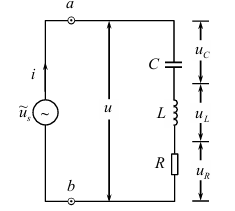
\includegraphics[width=0.4\textwidth]{rlc_series_circuit.png} % 替换为图1的实际文件名
    \caption{图1 RLC串联电路}
    \label{fig:rlc_series}
\end{figure}

1. 电路核心公式
电路总阻抗模值$|Z|$、电压$u$与电流$i$的相位差$\varphi$、回路电流$i$的表达式为：
\begin{align}
|Z| &= \sqrt{R^2 + \left( \omega L - \frac{1}{\omega C} \right)^2}, \tag{1} \\
\varphi &= \arctan \frac{\omega L - 1/(\omega C)}{R}, \tag{2} \\
i &= \frac{u}{\sqrt{R^2 + \left( \omega L - \frac{1}{\omega C} \right)^2}}, \tag{3}
\end{align}
其中$\omega = 2\pi f$为激励信号的角频率（$f$为频率）。可见$|Z|$、$\varphi$、$i$均为频率$f$的函数，电路特性由频率唯一决定。


2. 频率特性曲线
RLC串联电路的阻抗、相位、电流随频率的变化规律（频率特性）如图\ref{fig:rlc_series_freq}所示：
\begin{figure}[H]
    \centering
    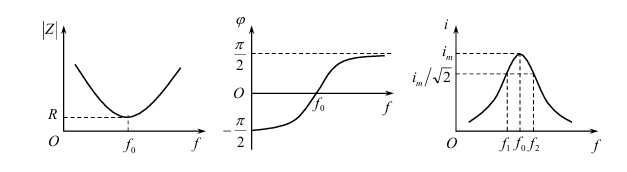
\includegraphics[width=0.8\textwidth]{rlc_series_freq_char.png} % 替换为图2的实际文件名
    \caption{图2 RLC串联电路的频率特性（a）阻抗特性；（b）相频特性；（c）幅频特性}
    \label{fig:rlc_series_freq}
\end{figure}


3. 串联谐振的核心特性
当$\omega L - 1/(\omega C) = 0$时，电路进入\textbf{串联谐振状态}，此时谐振角频率$\omega_0$（或谐振频率$f_0$）为：
\begin{equation}
\omega_0 = \frac{1}{\sqrt{LC}}, \quad f_0 = \frac{1}{2\pi \sqrt{LC}}, \tag{4}
\end{equation}
谐振状态的关键特征：
\begin{enumerate}[label={(\arabic*)}]
    \item 相位特性：$f < f_0$时$\varphi < 0$（电路呈容性），$f > f_0$时$\varphi > 0$（电路呈感性），谐振时$\varphi = 0$（纯阻性）；
    \item 阻抗与电流：谐振时总阻抗最小（$Z_0 = R$），回路电流最大（$i_m = u/R$）；
    \item 品质因数$Q$：定义为谐振时电感/电容电压与总电压的比值，是衡量谐振特性的核心参数：
    \begin{equation}
    Q = \frac{u_L}{u} = \frac{u_C}{u} = \frac{\omega_0 L}{R} = \frac{1}{R \omega_0 C}, \tag{5}
    \end{equation}
    $Q$值同时决定频率选择性：$Q = f_0/\Delta f$（$\Delta f = f_2 - f_1$为半功率带宽），$Q$越大，带宽越窄、选频能力越强。
\end{enumerate}


\subsection{并联谐振}
RLC并联电路结构如图\ref{fig:rlc_parallel}所示，其频率特性与串联电路呈互补关系。

\begin{figure}[H]
    \centering
    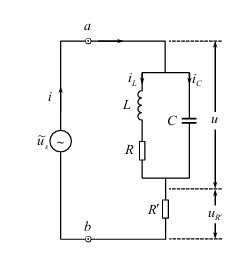
\includegraphics[width=0.4\textwidth]{rlc_parallel_circuit.png} % 替换为图3的实际文件名
    \caption{图3 RLC并联电路}
    \label{fig:rlc_parallel}
\end{figure}

1. 电路核心公式
并联电路的总阻抗模值$|Z_p|$、相位差$\varphi$、端电压$u$的表达式为：
\begin{align}
|Z_p| &= \sqrt{\frac{R^2 + (\omega L)^2}{\left( 1 - \omega^2 LC \right)^2 + (\omega CR)^2}}, \tag{7} \\
\varphi &= \arctan \frac{\omega L - \omega C \left[ R^2 + (\omega L)^2 \right]}{R}, \tag{8} \\
u &= i |Z_p| = \frac{u_{R'}}{R'} |Z_p|, \tag{9}
\end{align}


2. 并联谐振的核心特性
当$\varphi = 0$时电路进入\textbf{并联谐振状态}，谐振角频率$\omega_p$（或频率$f_p$）为：
\begin{equation}
\omega_p = \sqrt{\frac{1}{LC} - \left( \frac{R}{L} \right)^2} = \omega_0 \sqrt{1 - \frac{1}{Q^2}}, \tag{10}
\end{equation}
其中$\omega_0 = 1/\sqrt{LC}$为串联谐振角频率。当$Q \gg 1$时，$\omega_p \approx \omega_0$。

并联电路的频率特性如图\ref{fig:rlc_parallel_freq}所示，其核心特征与串联电路互补：谐振时总阻抗最大、总电流最小，电感/电容支路电流为总电流的$Q$倍（称为“电流谐振”）。

\begin{figure}[H]
    \centering
    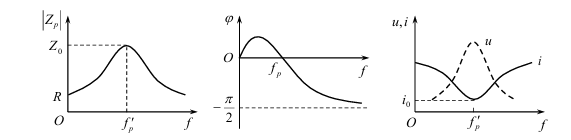
\includegraphics[width=0.8\textwidth]{rlc_parallel_freq_char.png} % 替换为图4的实际文件名
    \caption{图4 RLC并联电路的频率特性（a）阻抗特性；（b）相频特性；（c）幅频特性}
    \label{fig:rlc_parallel_freq}
\end{figure}


\subsection{RLC电路的暂态过程}
RLC电路的暂态过程（以电容充/放电为例）由二阶线性微分方程描述，电路结构如图\ref{fig:rlc_transient}所示。

\begin{figure}[H]
    \centering
    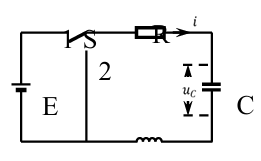
\includegraphics[width=0.4\textwidth]{rlc_transient_circuit.png} % 替换为图5的实际文件名
    \caption{图5 RLC暂态电路}
    \label{fig:rlc_transient}
\end{figure}

1. 放电过程的电路方程
电容放电时的电路方程为：
\begin{equation}
LC \frac{d^2 u_C}{dt^2} + RC \frac{du_C}{dt} + u_C = 0, \tag{12}
\end{equation}
结合初始条件$t=0$时$u_C = E$、$\frac{du_C}{dt}=0$，方程的解由阻尼系数$\zeta = \frac{R}{2}\sqrt{\frac{C}{L}}$决定，分为三种情况：

\begin{enumerate}[label={\Roman{enumi}}]
    \item \textbf{欠阻尼（$R^2 < 4L/C$，$\zeta < 1$）}：电路呈阻尼振动，电压响应为：
    \begin{equation}
    u_C = \sqrt{\frac{4L}{4L - R^2 C}} E e^{-t/\tau} \cos(\omega t + \varphi), \tag{13}
    \end{equation}
    其中时间常量$\tau = 2L/R$，衰减振动角频率$\omega = \frac{1}{\sqrt{LC}}\sqrt{1 - \frac{R^2 C}{4L}}$。

    \item \textbf{过阻尼（$R^2 > 4L/C$，$\zeta > 1$）}：电路无振动，电压缓慢衰减至零：
    \begin{equation}
    u_C = \sqrt{\frac{4L}{R^2 C - 4L}} E e^{-\alpha t} \sinh(\beta t + \varphi), \tag{18}
    \end{equation}
    其中$\alpha = R/(2L)$，$\beta = \frac{1}{\sqrt{LC}}\sqrt{\frac{R^2 C}{4L} - 1}$。

    \item \textbf{临界阻尼（$R^2 = 4L/C$，$\zeta = 1$）}：介于振动与非振动的临界状态，电压响应为：
    \begin{equation}
    u_C = E \left( 1 + \frac{t}{\tau} \right) e^{-t/\tau}, \tag{19}
    \end{equation}
\end{enumerate}


2. 充电过程的响应规律
电容充电时的电路方程为：
\begin{equation}
LC \frac{d^2 u_C}{dt^2} + RC \frac{du_C}{dt} + u_C = E, \tag{20}
\end{equation}
其解的形式与放电过程类似，仅平衡位置由“0”变为“$E$”，三种阻尼下的响应曲线如图\ref{fig:rlc_transient_damping}所示。

\begin{figure}[H]
    \centering
    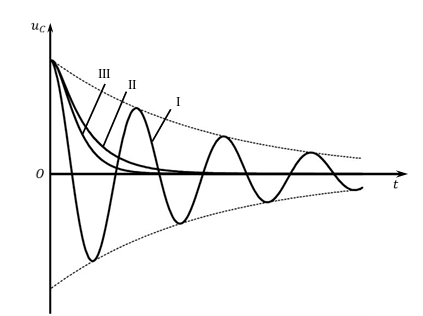
\includegraphics[width=0.6\textwidth]{rlc_transient_damping.png} % 替换为图6的实际文件名
    \caption{RLC暂态过程中的三种阻尼曲线}
    \label{fig:rlc_transient_damping}
\end{figure}

\section{实验内容}
本实验分为RLC串联电路频率特性测量、RLC并联电路频率特性测量、RLC串联暂态过程观测三部分，各部分实验参数与操作流程如下：

\subsection{RLC串联电路相频特性与幅频特性曲线测量}
本部分通过观测串联电路的电压相位差与电流幅值，获取其频率响应特性，固定实验参数为：$L=0.1\,\text{H}$，$C=0.05\,\mu\text{F}$，$R=100\,\Omega$。

\begin{figure}[H]
    \centering
    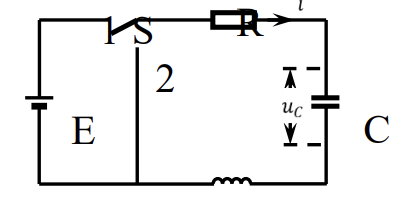
\includegraphics[width=0.5\textwidth]{rlc_series_exp_circuit.png} % 替换为图7的实际文件名
    \caption{RLC串联电路实验连接图}
    \label{fig:exp_series}
\end{figure}

\begin{enumerate}
    \item \textbf{电路连接与谐振点定位} \\
    按照图\ref{fig:exp_series}连接电路：示波器CH1通道测量路端总电压$u$，CH2通道测量电阻$R$的电压$u_R$（用于间接反映回路电流，因$i=u_R/R$）。
    
    操作要点：
    \begin{itemize}
        \item 确保示波器与函数发生器共地，避免信号干扰；
        \item 调节函数发生器频率，当CH1与CH2的相位差为0、且CH2幅值达到最大时，电路处于串联谐振状态，记录此时的谐振频率$f_0$。
    \end{itemize}

    \item \textbf{品质因数$Q$的测量} \\
    保持电路处于谐振状态，使用数字多用表交流电压档，分别测量电感端电压$u_L$、电容端电压$u_C$及路端总电压$u$，利用串联谐振时$Q=u_L/u=u_C/u$计算电路品质因数。
    
    注意：万用表测量值为电压有效值，与示波器显示的峰峰值（Vpp）需区分（有效值$U=\text{Vpp}/(2\sqrt{2})$）。

    \item \textbf{频率特性曲线的测绘} \\
    保持示波器CH1的路端电压峰峰值稳定在$2\,\text{V}$（不同频率下需微调函数发生器输出，维持CH1幅值在$1.99\sim2.01\,\text{V}$之间），选取包含谐振频率$f_0$的若干频率点，依次测量：
    \begin{itemize}
        \item CH1与CH2的相位差（反映电路相频特性）；
        \item CH2的幅值（反映回路电流幅值，对应幅频特性）。
    \end{itemize}
    将测量数据整理后，绘制RLC串联电路的相频特性曲线与幅频特性曲线。
\end{enumerate}

\subsection{RLC并联电路相频特性与幅频特性曲线测量}
本部分观测并联电路的频率响应特性，固定实验参数为：$L=0.1\,\text{H}$，$C=0.05\,\mu\text{F}$，取样电阻$R'=5\,\text{k}\Omega$（电感内阻无需额外连接）。

\begin{figure}[H]
    \centering
    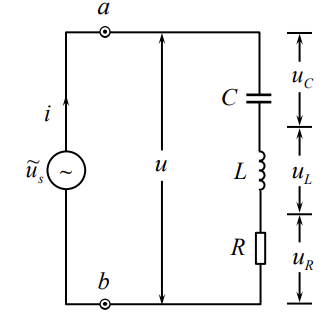
\includegraphics[width=0.5\textwidth]{rlc_parallel_exp_circuit.png} % 替换为图8的实际文件名
    \caption{RLC并联电路实验连接图}
    \label{fig:exp_parallel}
\end{figure}

\begin{enumerate}
    \item \textbf{电路连接与谐振点定位} \\
    按照图\ref{fig:exp_parallel}连接电路：示波器CH1通道测量路端总电压，CH2通道测量取样电阻$R'$的电压$u_{R'}$；利用示波器MATH功能计算“CH1-CH2”，得到并联支路的端电压$u$（显示为紫色信号线）。
    
    操作要点：
    \begin{itemize}
        \item 调节函数发生器频率，当“CH1-CH2”与CH2的相位差为0、且CH2幅值达到最小时，电路处于并联谐振状态（此时总阻抗最大、总电流最小），记录此时的谐振频率$f_p$。
    \end{itemize}

    \item \textbf{频率特性曲线的测绘} \\
    保持示波器CH1的总电压峰峰值稳定在$2\,\text{V}$（不同频率下微调函数发生器输出），选取包含$f_p$的若干频率点，依次测量：
    \begin{itemize}
        \item “CH1-CH2”与CH2的相位差（反映电路相频特性）；
        \item “CH1-CH2”的幅值（并联支路电压$u$）与CH2的幅值（$u_{R'}$，反映总电流）。
    \end{itemize}
    利用相位差计算公式$\varphi = \frac{\Delta t}{T} \times 360^\circ = \frac{f}{1/\Delta t} \times 360^\circ$（其中$\Delta t$为相位差对应的时间差，$T$为信号周期），将数据整理后绘制并联电路的相频、幅频特性曲线。
\end{enumerate}

\subsection{RLC串联电路暂态过程观测}
本部分通过方波激励模拟阶跃信号，观测不同阻尼条件下电容电压的暂态响应，固定实验参数为：$C=0.2\,\mu\text{F}$，$L=0.1\,\text{H}$。

\begin{figure}[H]
    \centering
    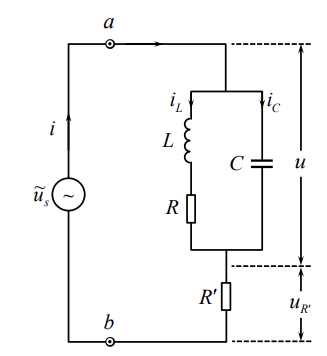
\includegraphics[width=0.4\textwidth]{rlc_transient_exp_circuit.png} % 替换为图9的实际文件名
    \caption{RLC串联暂态电路实验连接图}
    \label{fig:exp_transient}
\end{figure}

\begin{enumerate}
    \item \textbf{电路连接与激励信号设置} \\
    按照图\ref{fig:exp_transient}连接电路，函数发生器输出方波信号（模拟阶跃激励），参数设置为：频率$f=50\,\text{Hz}$，峰峰值$\text{Vpp}=2.0\,\text{V}$。
    示波器连接：CH1通道测量总电压，CH2通道测量电容端电压$u_C$，注意两通道共地以避免信号失真。

    \item \textbf{不同阻尼条件下的暂态波形观测} \\
    通过电阻箱调节串联电阻$R$的阻值，分别观测以下阻尼状态下$u_C$的波形：
    \begin{itemize}
        \item 欠阻尼状态（$R^2 < 4L/C$）：$u_C$呈衰减振动波形；
        \item 过阻尼状态（$R^2 > 4L/C$）：$u_C$无振动、缓慢衰减至稳态；
        \item 临界阻尼状态（$R^2 = 4L/C$）：$u_C$以最快速度衰减至稳态（无振动）。
    \end{itemize}

    \item \textbf{临界电阻的测量与验证} \\
    测量使电路处于临界阻尼状态的电阻值（临界电阻$R_{\text{cr}} = 2\sqrt{L/C}$），并与理论值$R_{\text{cr}}=2\sqrt{0.1/(0.2\times10^{-6})}=1000\,\Omega$对比，分析实验误差来源。

    \item \textbf{数据存储} \\
    利用数字存储示波器的波形存储功能（或拍照），记录不同阻尼状态下$u_C$的暂态波形，用于后续分析。
\end{enumerate}


\section{实验数据与分析}
\subsection{RLC串联电路实验数据与分析}

\subsubsection{实验数据与特性曲线}
串联电路的实验测量数据如表\ref{tab:series1_data}所示。根据表格数据，绘制电路的相频特性曲线与幅频特性曲线如图\ref{fig:series_char}所示。

\begin{table}[htbp]
    \centering
    \caption{实验数据表格}
    \label{tab:series1_data}
    \begin{tabular}{
        S[table-format=1.3]  % f/kHz（1位整数，3位小数）
        S[table-format=1.0]  % U(pp)/V（整数）
        S[table-format=-2.2] % (CH1-CH2)phi/°（带负号，2位整数，2位小数）
        S[table-format=1.4]  % U\_R(Vamp)/V（1位整数，4位小数）
        S[table-format=1.3]  % I\_MAX/mA（1位整数，3位小数）
    }
        \toprule
        {$f/\si{\kilo\hertz}$} & {$U(\text{pp})/\si{\volt}$} & {$\varphi_{(\text{CH1-CH2})}/\si{\degree}$} & {$U_R(\text{Vamp})/\si{\volt}$} & {$I_{\text{MAX}}/\si{\milli\ampere}$} \\
        \midrule
        1.88   & 2 & -77.82 & 0.175  & 1.75   \\
        2.00   & 2 & -68.19 & 0.2273 & 2.273  \\
        2.08    & 2 & -59.8  & 0.3807 & 3.807  \\
        2.15   & 2 & -46.55 & 0.5336 & 5.336  \\
        2.19   & 2 & -32    & 0.652  & 6.52   \\
        2.22   & 2 & -15.76 & 0.719  & 7.19   \\
        2.24   & 2 & -6.52  & 0.7564 & 7.564  \\
        2.25   & 2 & -2.43  & 0.7603 & 7.603  \\
        2.26   & 2 & 4.61   & 0.7359 & 7.359  \\
        2.275  & 2 & 12.2   & 0.7431 & 7.431  \\
        2.3    & 2 & 25     & 0.6292 & 6.292  \\
        2.36   & 2 & 44.23  & 0.4849 & 4.849  \\
        2.43   & 2 & 57.09  & 0.3303 & 3.303  \\
        2.62   & 2 & 69.02  & 0.195  & 1.95   \\
        3.18   & 2 & 76.84 & 0.1155 & 1.155  \\
        \bottomrule
    \end{tabular}
\end{table}

\begin{figure}[htbp]
    \centering
    \begin{subfigure}[b]{0.48\textwidth}
        \centering
        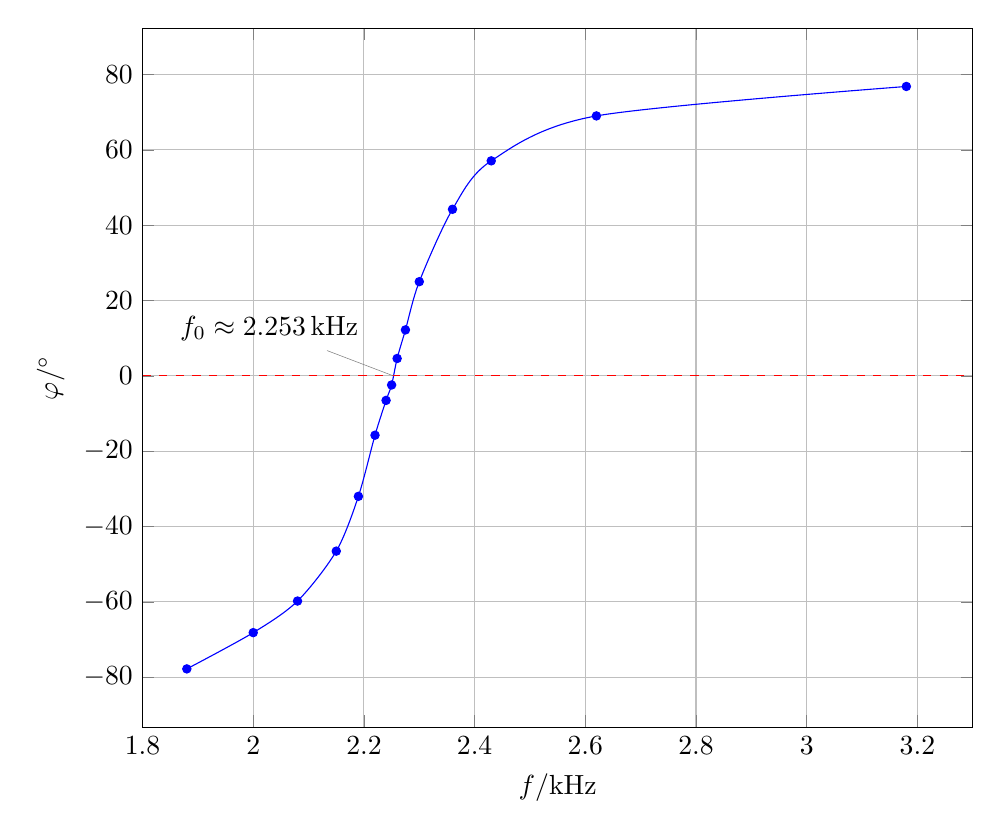
\begin{tikzpicture}
            \begin{axis}[
                xlabel={$f/\si{\kilo\hertz}$},
                ylabel={$\varphi/\si{\degree}$},
                grid=major,
                width=\textwidth,
                xmin=1.8, xmax=3.3,
            ]
            \addplot[smooth, mark=*, mark size=1.5pt, blue] coordinates {
                (1.88, -77.82) (2.00, -68.19) (2.08, -59.8) (2.15, -46.55) (2.19, -32)
                (2.22, -15.76) (2.24, -6.52) (2.25, -2.43) (2.26, 4.61) (2.275, 12.2)
                (2.3, 25) (2.36, 44.23) (2.43, 57.09) (2.62, 69.02) (3.18, 76.84)
            };
            \draw[red, dashed] (axis cs:1.8,0) -- (axis cs:3.3,0);
            \node[coordinate, pin=135:{$f_0 \approx 2.253\,\si{\kilo\hertz}$}] at (axis cs:2.253, 0) {};
            \end{axis}
        \end{tikzpicture}
        \caption{相频特性曲线}
    \end{subfigure}
    \hfill
    \begin{subfigure}[b]{0.48\textwidth}
        \centering
        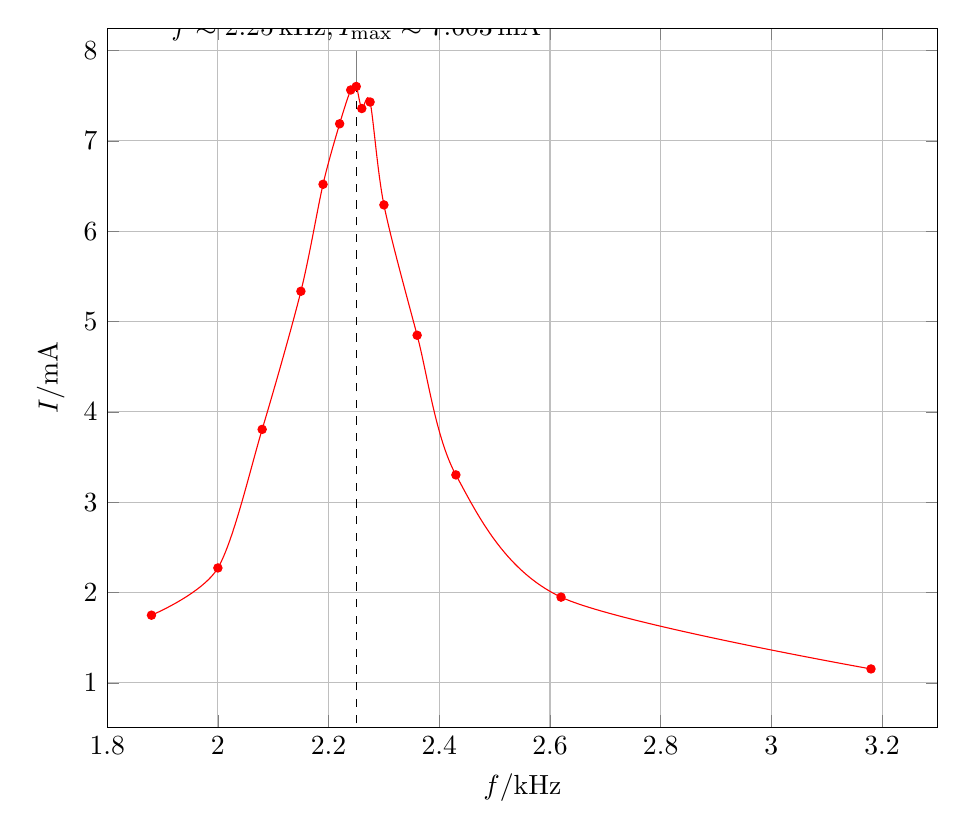
\begin{tikzpicture}
            \begin{axis}[
                xlabel={$f/\si{\kilo\hertz}$},
                ylabel={$I/\si{\milli\ampere}$},
                grid=major,
                width=\textwidth,
                xmin=1.8, xmax=3.3,
            ]
            \addplot[smooth, mark=*, mark size=1.5pt, red] coordinates {
                (1.88, 1.75) (2.00, 2.273) (2.08, 3.807) (2.15, 5.336) (2.19, 6.52)
                (2.22, 7.19) (2.24, 7.564) (2.25, 7.603) (2.26, 7.359) (2.275, 7.431)
                (2.3, 6.292) (2.36, 4.849) (2.43, 3.303) (2.62, 1.95) (3.18, 1.155)
            };
            \draw[dashed] (axis cs:2.25, 0) -- (axis cs:2.25, 7.603);
            \node[coordinate, pin=90:{$f \approx 2.25\,\si{\kilo\hertz}, I_{\max} \approx 7.603\,\si{\milli\ampere}$}] at (axis cs:2.25, 7.603) {};
            \end{axis}
        \end{tikzpicture}
        \caption{幅频特性曲线}
    \end{subfigure}
    \caption{RLC串联电路频率特性曲线}
    \label{fig:series_char}
\end{figure}

\subsubsection{数据分析}
\begin{enumerate}
    \item \textbf{谐振频率与电压比法求Q值}
    
    调节信号源频率，观测到电路发生串联谐振的频率为$f_0=2.248\,\text{kHz}$。
    此时测得电感端电压$u_C=5.52\,\text{V}$（有效值），路端总电压$U=0.472\,\text{V}$。
    根据品质因数定义计算：
    \[ Q_1 = \frac{u_C}{U} = \frac{5.52}{0.472} \approx 11.7 \]

    \item \textbf{频带宽度法求Q值}
    
    由幅频特性曲线可知，谐振电流最大值$I_{\max} = 7.603\,\text{mA}$。
    半功率点电流对应值为$I_{1/\sqrt{2}} = I_{\max}/\sqrt{2} \approx 5.376\,\text{mA}$。
    
    根据表\ref{tab:series1_data}数据，通过线性插值确定半功率点频率：
    \begin{itemize}
        \item 下半功率点：$f=2.15\,\text{kHz}$时$I=5.336\,\text{mA}$，接近$I_{1/\sqrt{2}}$，故取$f_1 \approx 2.15\,\text{kHz}$。
        \item 上半功率点：$I_{1/\sqrt{2}}$位于$2.30\,\text{kHz}$与$2.36\,\text{kHz}$之间。
        \[ f_2 \approx 2.30 + \frac{5.376 - 6.292}{4.849 - 6.292} \times (2.36 - 2.30) \approx 2.338\,\text{kHz} \]
    \end{itemize}
    
    通频带宽度 $\Delta f = f_2 - f_1 = 2.338 - 2.15 = 0.188\,\text{kHz}$。
    由此计算品质因数（取中心频率$f_0 \approx 2.25\,\text{kHz}$）：
    \[ Q_2 = \frac{f_0}{\Delta f} = \frac{2.25}{0.188} \approx 11.97 \]
\end{enumerate}

\subsubsection{实验总结}
\begin{enumerate}
    \item \textbf{谐振现象验证}：实验结果清晰展示了RLC串联电路的谐振特性。在谐振频率$f_0$附近，回路电流达到最大值，且电压与电流相位差为零（电路呈纯阻性）。当$f<f_0$时，相位差为负（容性）；当$f>f_0$时，相位差为正（感性）。
    
    \item \textbf{Q值一致性分析}：通过电压比法测得的$Q_1 \approx 11.7$与通过频带宽度法测得的$Q_2 \approx 11.97$高度一致，相对误差约为$2.3\%$。这表明实验数据准确可靠，且验证了品质因数不同定义在实际电路中的等效性。
    
    \item \textbf{误差来源}：实验值与理论预期（如理想$L,C$参数计算值）的微小偏差，主要归因于电感线圈存在的直流内阻、电容的损耗角正切以及连接导线的分布参数影响。
\end{enumerate} 

\subsection{RLC并联电路实验数据与分析}

\subsubsection{实验数据与特性曲线}
并联电路的实验测量数据如表\ref{tab:rlc_parallel_data}所示。根据表格数据，绘制电路的相频特性曲线与幅频特性曲线如图\ref{fig:parallel_char}所示。

\begin{table}[htbp]
    \centering
    \caption{RLC并联电路测试数据（\(U_{\text{pp}}=2\,\text{V}\)）}
    \label{tab:rlc_parallel_data}
    \begin{tabular}{
        S[table-format=1.3]  % f/kHz
        S[table-format=1.0]  % Upp/V
        S[table-format=3.0]  % dt/us
        S[table-format=2.2]  % phi/deg
        S[table-format=3.1]  % u_branch/V
        S[table-format=3.1]  % u_R/mV
        S[table-format=1.3]  % I/mA
    }
        \toprule
        {$f/\si{\kilo\hertz}$} & {$U_{\text{pp}}/\si{\volt}$} & {$\delta t/\si{\micro\second}$} & {$\phi/\si{\degree}$} & {$u_{\text{CH1-CH2}}/\si{\volt}$} & {$u_R/\si{\milli\volt}$} & {$I_{\text{MAX}}/\si{\milli\ampere}$} \\
        \midrule
        2.050 & 2 & 115 & 84.87 & 359.6 & 846.2 & 0.169 \\
        2.150 & 2 & 116 & 89.78 & 515.6 & 647.3 & 0.129 \\
        2.200 & 2 & 98  & 77.62 & 599.5 & 484.1 & 0.097 \\
        2.231 & 2 & 68  & 54.61 & 679.1 & 300.5 & 0.060 \\
        2.240 & 2 & 56  & 45.16 & 720.4 & 262.1 & 0.052 \\
        2.247 & 2 & 32  & 25.89 & 716.1 & 228.0 & 0.046 \\
        2.250 & 2 & 14  & 11.34 & 725.6 & 229.0 & 0.046 \\
        2.253 & 2 & 6   & 4.87  & 758.7 & 205.3 & 0.041 \\
        2.256 & 2 & 8   & 6.50  & 764.5 & 217.6 & 0.044 \\
        2.265 & 2 & 38  & 30.99 & 763.1 & 219.1 & 0.044 \\
        2.275 & 2 & 46  & 37.67 & 728.0 & 296.4 & 0.059 \\
        2.320 & 2 & 84  & 70.16 & 613.9 & 590.9 & 0.118 \\
        2.400 & 2 & 98  & 84.67 & 364.6 & 800.0 & 0.160 \\
        2.600 & 2 & 18  & 16.85 & 197.4 & 898.4 & 0.180 \\
        \bottomrule
    \end{tabular}
\end{table}

\begin{figure}[htbp]
    \centering
    \begin{subfigure}[b]{0.48\textwidth}
        \centering
        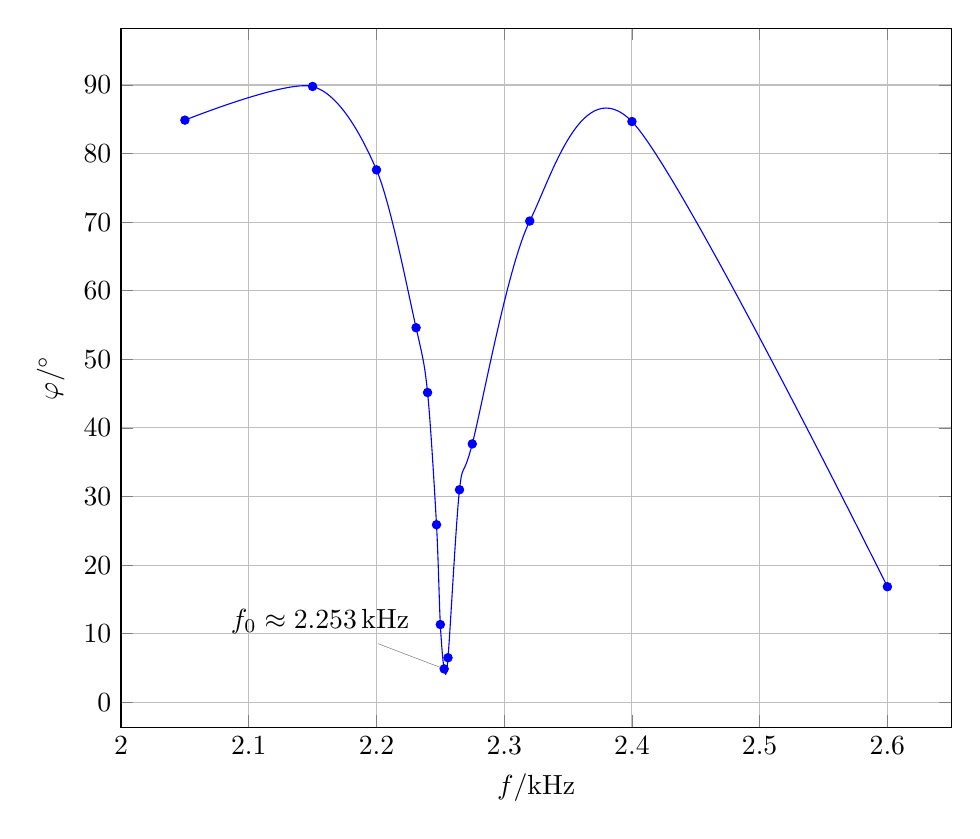
\begin{tikzpicture}
            \begin{axis}[
                xlabel={$f/\si{\kilo\hertz}$},
                ylabel={$\varphi/\si{\degree}$},
                grid=major,
                width=\textwidth,
                xmin=2.0, xmax=2.65,
            ]
            \addplot[smooth, mark=*, mark size=1.5pt, blue] coordinates {
                (2.050, 84.87) (2.150, 89.78) (2.200, 77.62) (2.231, 54.61) (2.240, 45.16)
                (2.247, 25.89) (2.250, 11.34) (2.253, 4.87) (2.256, 6.50) (2.265, 30.99)
                (2.275, 37.67) (2.320, 70.16) (2.400, 84.67) (2.600, 16.85)
            };
            \node[coordinate, pin=135:{$f_0 \approx 2.253\,\si{\kilo\hertz}$}] at (axis cs:2.253, 4.87) {};
            \end{axis}
        \end{tikzpicture}
        \caption{相频特性曲线}
    \end{subfigure}
    \hfill
    \begin{subfigure}[b]{0.48\textwidth}
        \centering
        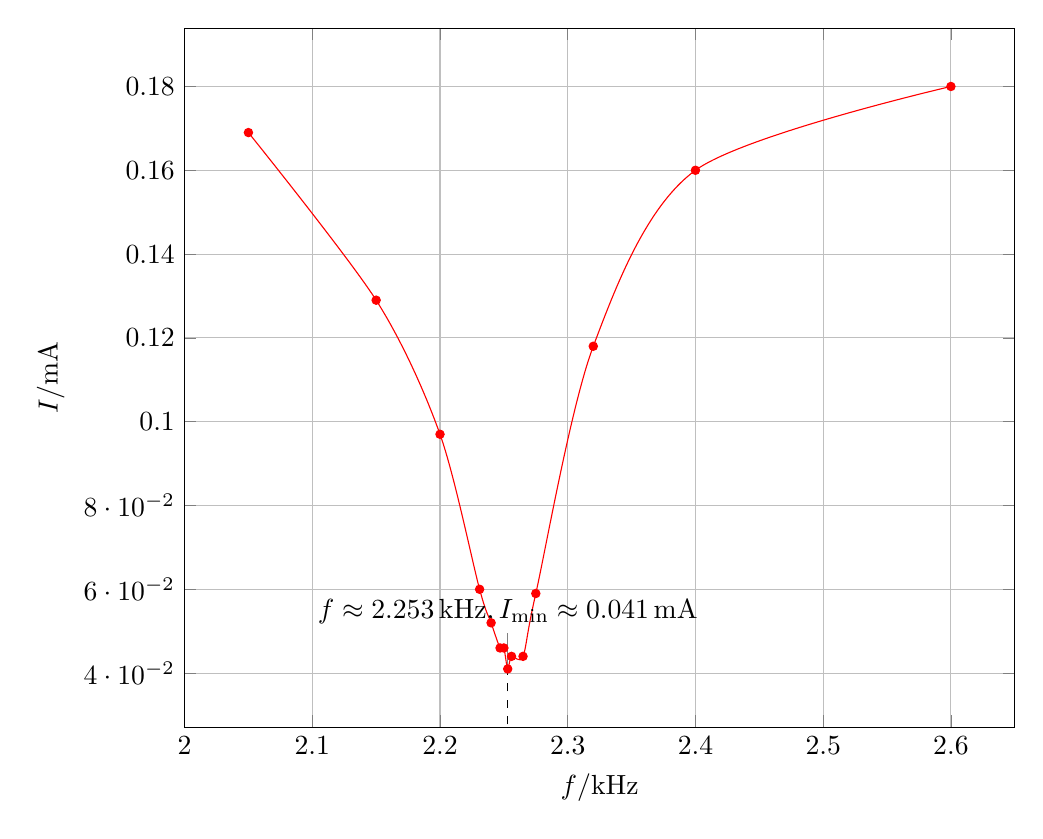
\begin{tikzpicture}
            \begin{axis}[
                xlabel={$f/\si{\kilo\hertz}$},
                ylabel={$I/\si{\milli\ampere}$},
                grid=major,
                width=\textwidth,
                xmin=2.0, xmax=2.65,
            ]
            \addplot[smooth, mark=*, mark size=1.5pt, red] coordinates {
                (2.050, 0.169) (2.150, 0.129) (2.200, 0.097) (2.231, 0.060) (2.240, 0.052)
                (2.247, 0.046) (2.250, 0.046) (2.253, 0.041) (2.256, 0.044) (2.265, 0.044)
                (2.275, 0.059) (2.320, 0.118) (2.400, 0.160) (2.600, 0.180)
            };
            \draw[dashed] (axis cs:2.253, 0) -- (axis cs:2.253, 0.041);
            \node[coordinate, pin=90:{$f \approx 2.253\,\si{\kilo\hertz}, I_{\min} \approx 0.041\,\si{\milli\ampere}$}] at (axis cs:2.253, 0.041) {};
            \end{axis}
        \end{tikzpicture}
        \caption{幅频特性曲线}
    \end{subfigure}
    \caption{RLC并联电路频率特性曲线}
    \label{fig:parallel_char}
\end{figure}

\subsubsection{数据分析}
\begin{enumerate}
    \item \textbf{谐振频率}
    
    由幅频特性曲线及实验数据可知，当频率调节至$f_0=2.253\,\text{kHz}$时，回路总电流达到最小值$I_{\min}=0.041\,\text{mA}$，且此时电压与电流相位差接近最小值（约为$4.87^\circ$），判定电路处于并联谐振状态。

    \item \textbf{频带宽度法求Q值}
    
    并联谐振时总电流最小，半功率点对应于总阻抗下降至$1/\sqrt{2}$倍，即总电流上升至$\sqrt{2}$倍。
    \[ I_{1/\sqrt{2}} = \sqrt{2} I_{\min} = \sqrt{2} \times 0.041 \approx 0.058\,\text{mA} \]
    
    根据表\ref{tab:rlc_parallel_data}数据，通过线性插值确定半功率点频率：
    \begin{itemize}
        \item 下半功率点：$I$在$2.231\,\text{kHz}$ ($0.060\,\text{mA}$)与$2.240\,\text{kHz}$ ($0.052\,\text{mA}$)之间。
        \[ f_1 \approx 2.231 + \frac{0.058 - 0.060}{0.052 - 0.060} \times (2.240 - 2.231) \approx 2.233\,\text{kHz} \]
        \item 上半功率点：$I$在$2.265\,\text{kHz}$ ($0.044\,\text{mA}$)与$2.275\,\text{kHz}$ ($0.059\,\text{mA}$)之间。
        \[ f_2 \approx 2.265 + \frac{0.058 - 0.044}{0.059 - 0.044} \times (2.275 - 2.265) \approx 2.274\,\text{kHz} \]
    \end{itemize}
    
    通频带宽度 $\Delta f = f_2 - f_1 = 2.274 - 2.233 = 0.041\,\text{kHz}$。
    由此计算并联电路的品质因数：
    \[ Q = \frac{f_0}{\Delta f} = \frac{2.253}{0.041} \approx 54.95 \]
\end{enumerate}

\subsubsection{实验总结}
\begin{enumerate}
    \item \textbf{并联谐振特性}：实验结果验证了RLC并联电路的“电流谐振”特性。在谐振频率附近，总电流出现显著的极小值，表明电路总阻抗达到最大。
    
    \item \textbf{高Q值特性}：测得并联电路的品质因数$Q \approx 55$，显著高于串联电路实验中的Q值（约12）。这是因为串联实验中人为串入了$100\,\Omega$电阻，而并联实验中谐振回路（电感与电容并联）未串入额外电阻，其损耗主要来自电感线圈的直流内阻，故损耗较小，Q值较高，谐振曲线更为尖锐，选频特性更好。
\end{enumerate}
\subsection{RLC串联电路暂态过程实验数据与分析}

\subsubsection{实验数据与波形}
本实验通过数字存储示波器观测RLC串联电路在方波激励下的电容电压波形，实验参数设定如表\ref{tab:rlc_transient_params}所示。不同阻尼状态下的实验波形如图\ref{fig:rlc_transient_waveforms}所示。

\begin{table}[htbp]
    \centering
    \caption{RLC串联暂态过程实验参数表}
    \label{tab:rlc_transient_params}
    \begin{tabular}{cccccc}
        \toprule
        {电感 $L$} & {电容 $C$} & {电阻 $R$} & {激励频率 $f$} & {暂态类型} & {观测目标} \\
        \midrule
        \SI{0.1}{\henry} & \SI{0.2}{\micro\farad} & \SI{0}{\ohm} & \SI{50}{\hertz} & 欠阻尼 & 振荡衰减 \\
        \SI{0.1}{\henry} & \SI{0.2}{\micro\farad} & \SI{2}{\kilo\ohm} & \SI{250}{\hertz} & 过阻尼 & 缓慢衰减 \\
        \SI{0.1}{\henry} & \SI{0.2}{\micro\farad} & \SI{20}{\kilo\ohm} & \SI{20}{\hertz} & 强过阻尼 & 极慢衰减 \\
        \bottomrule
    \end{tabular}
\end{table}

\begin{figure}[htbp]
    \centering
    \begin{subfigure}[b]{0.32\textwidth}
        \centering
        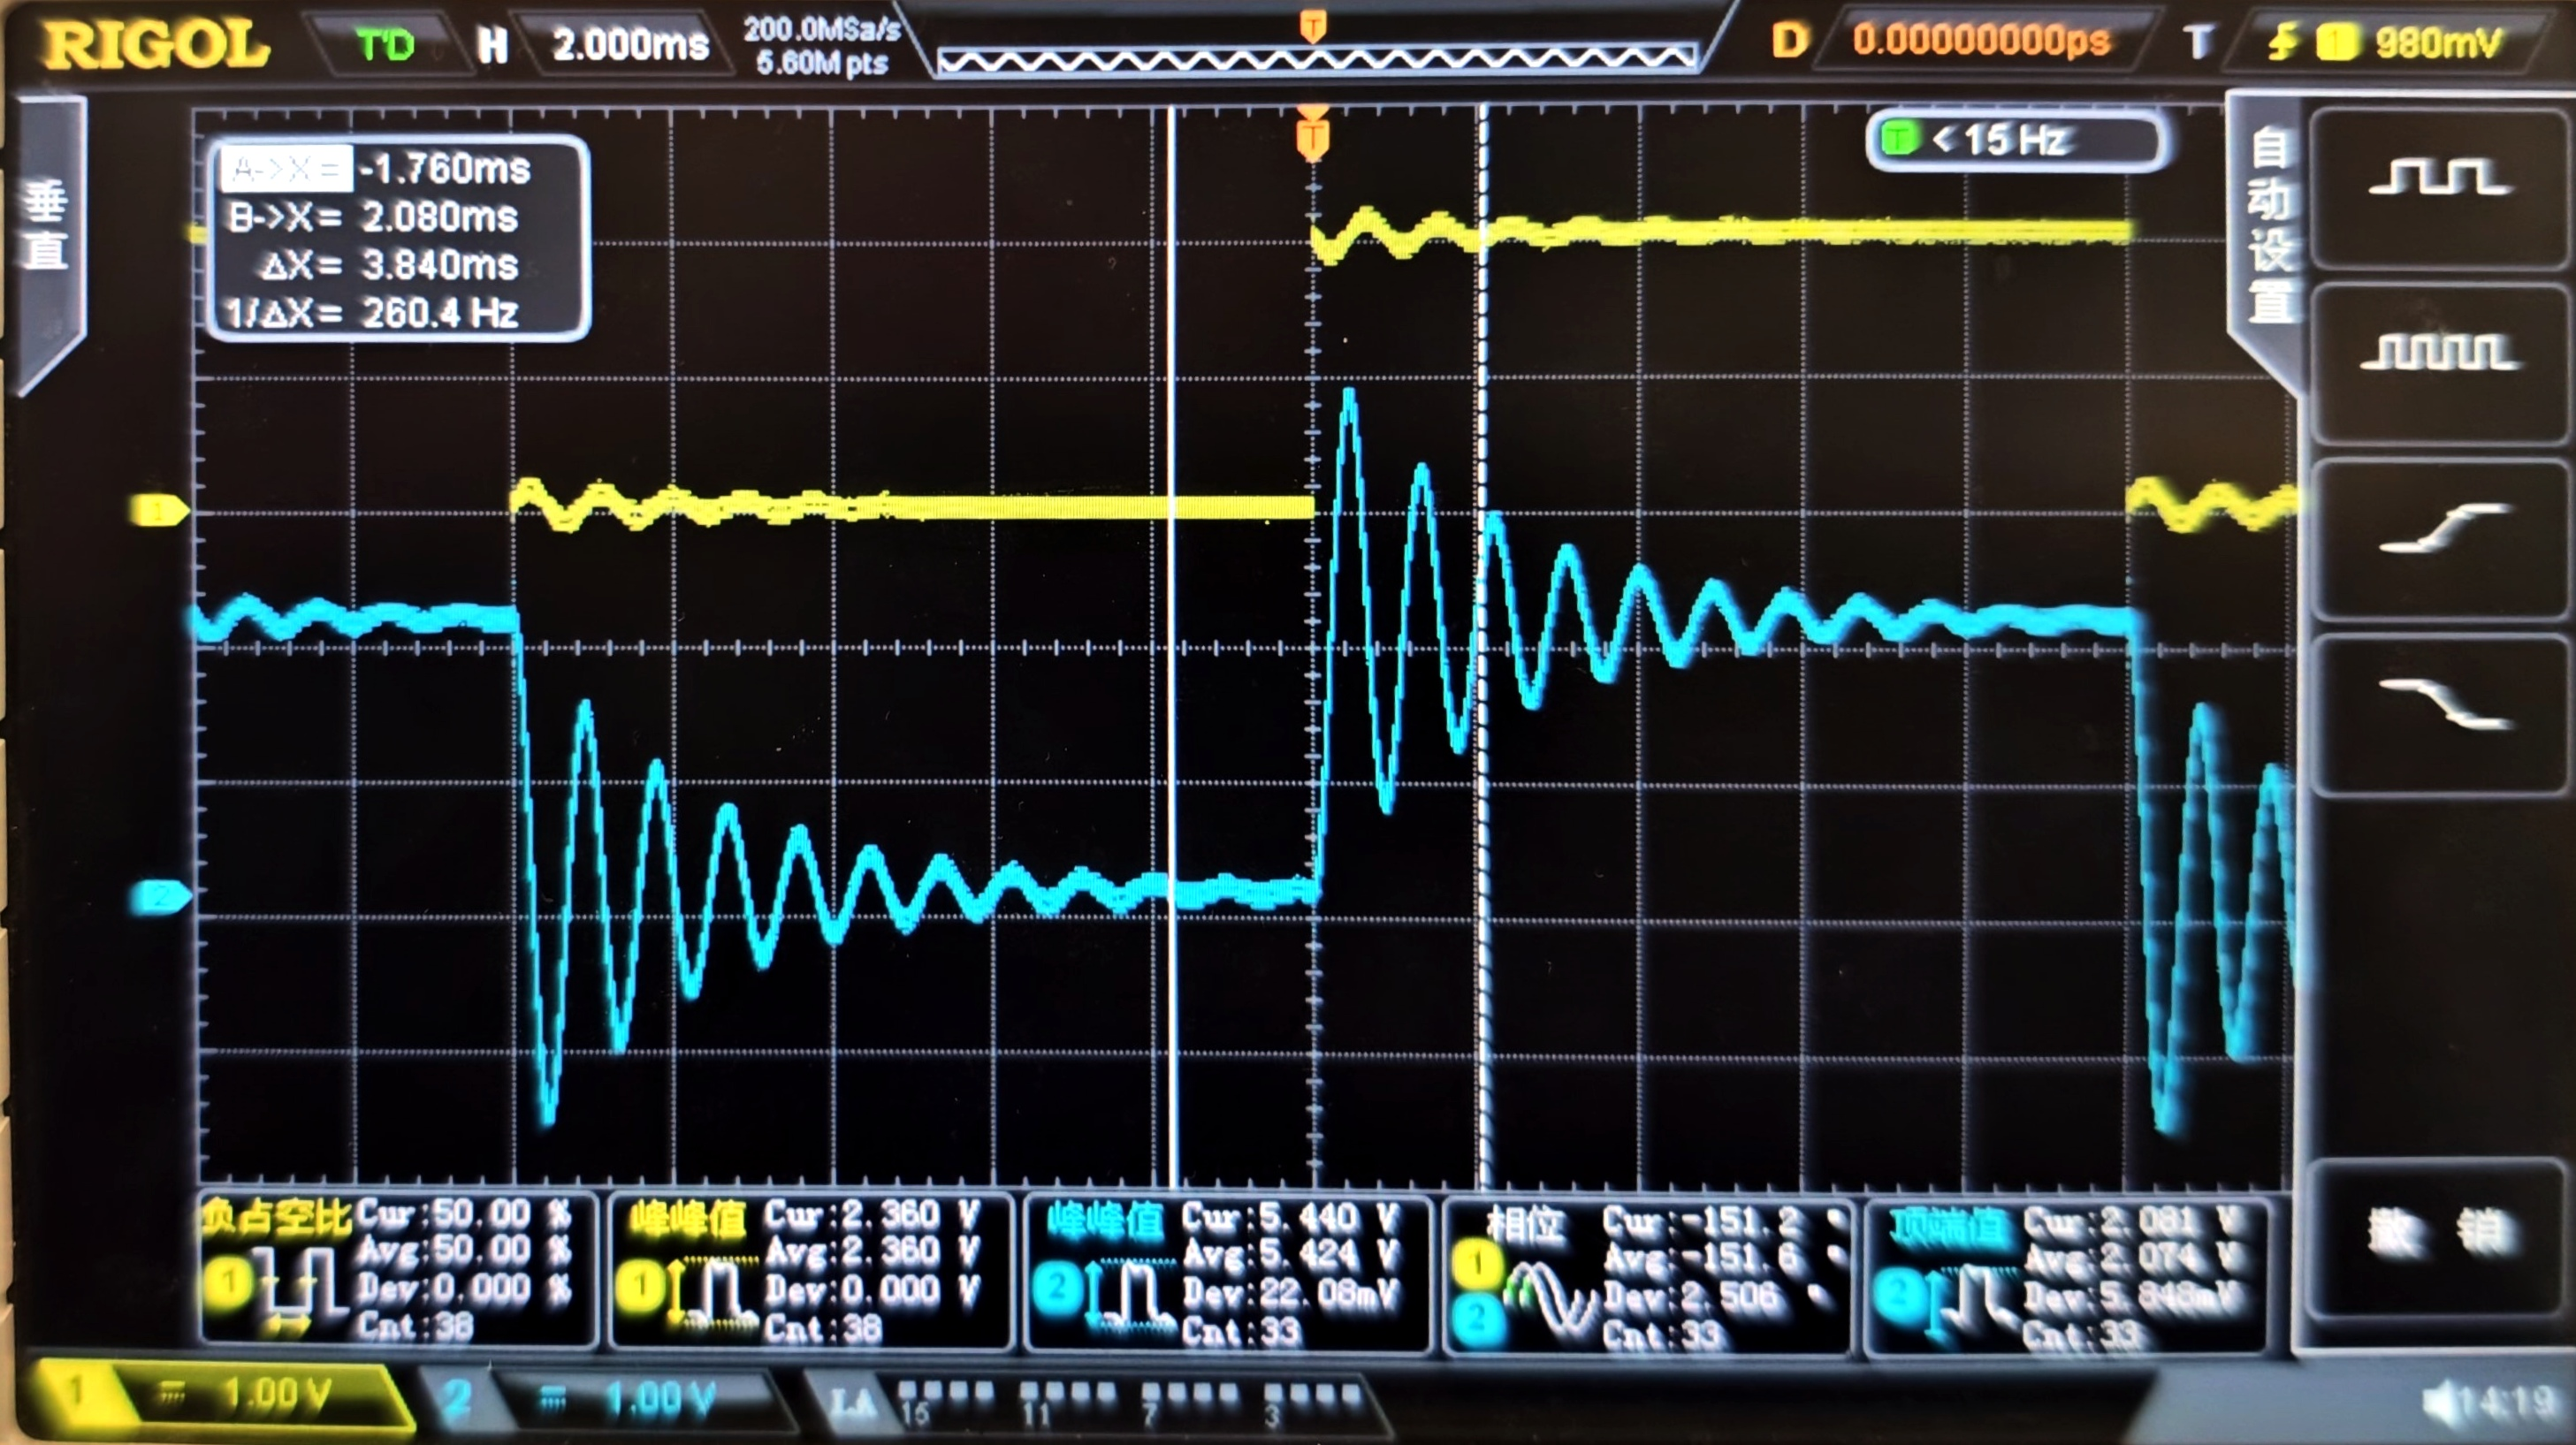
\includegraphics[width=\textwidth]{rlc_transient_R0.jpg}
        \caption{欠阻尼 ($R=\SI{0}{\ohm}$)}
        \label{fig:rlc_trans_R0}
    \end{subfigure}
    \hfill
    \begin{subfigure}[b]{0.32\textwidth}
        \centering
        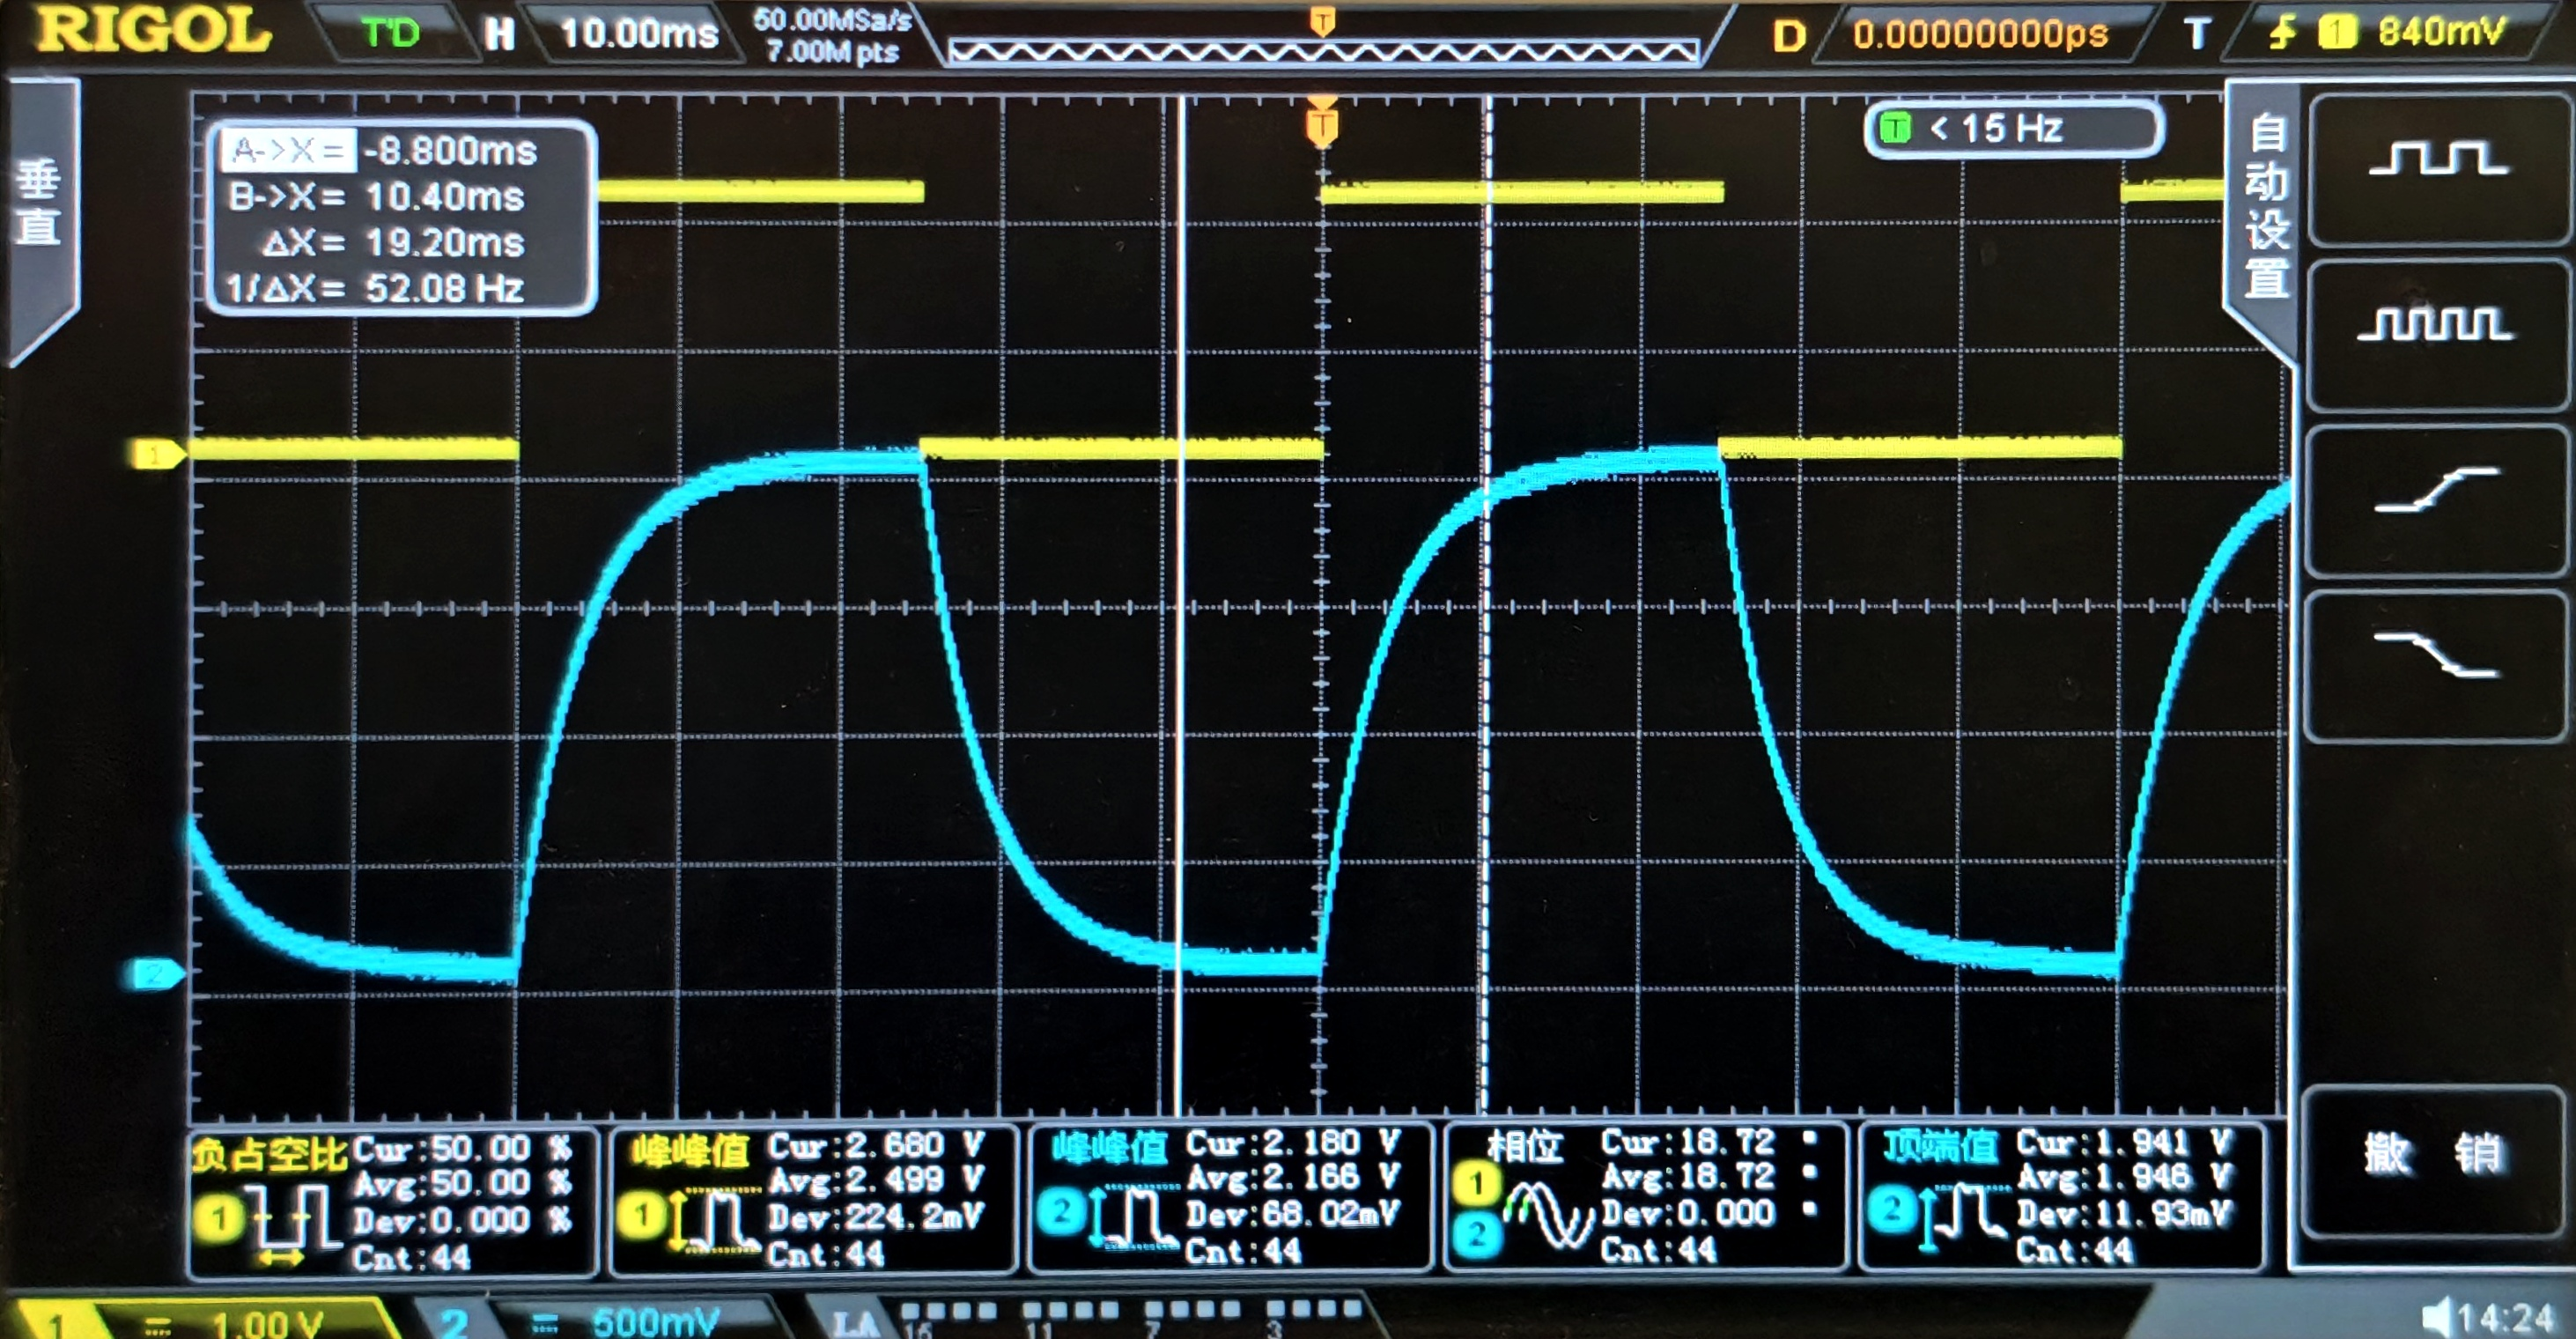
\includegraphics[width=\textwidth]{rlc_transient_R2k.jpg}
        \caption{过阻尼 ($R=\SI{2}{\kilo\ohm}$)}
        \label{fig:rlc_trans_R2k}
    \end{subfigure}
    \hfill
    \begin{subfigure}[b]{0.32\textwidth}
        \centering
        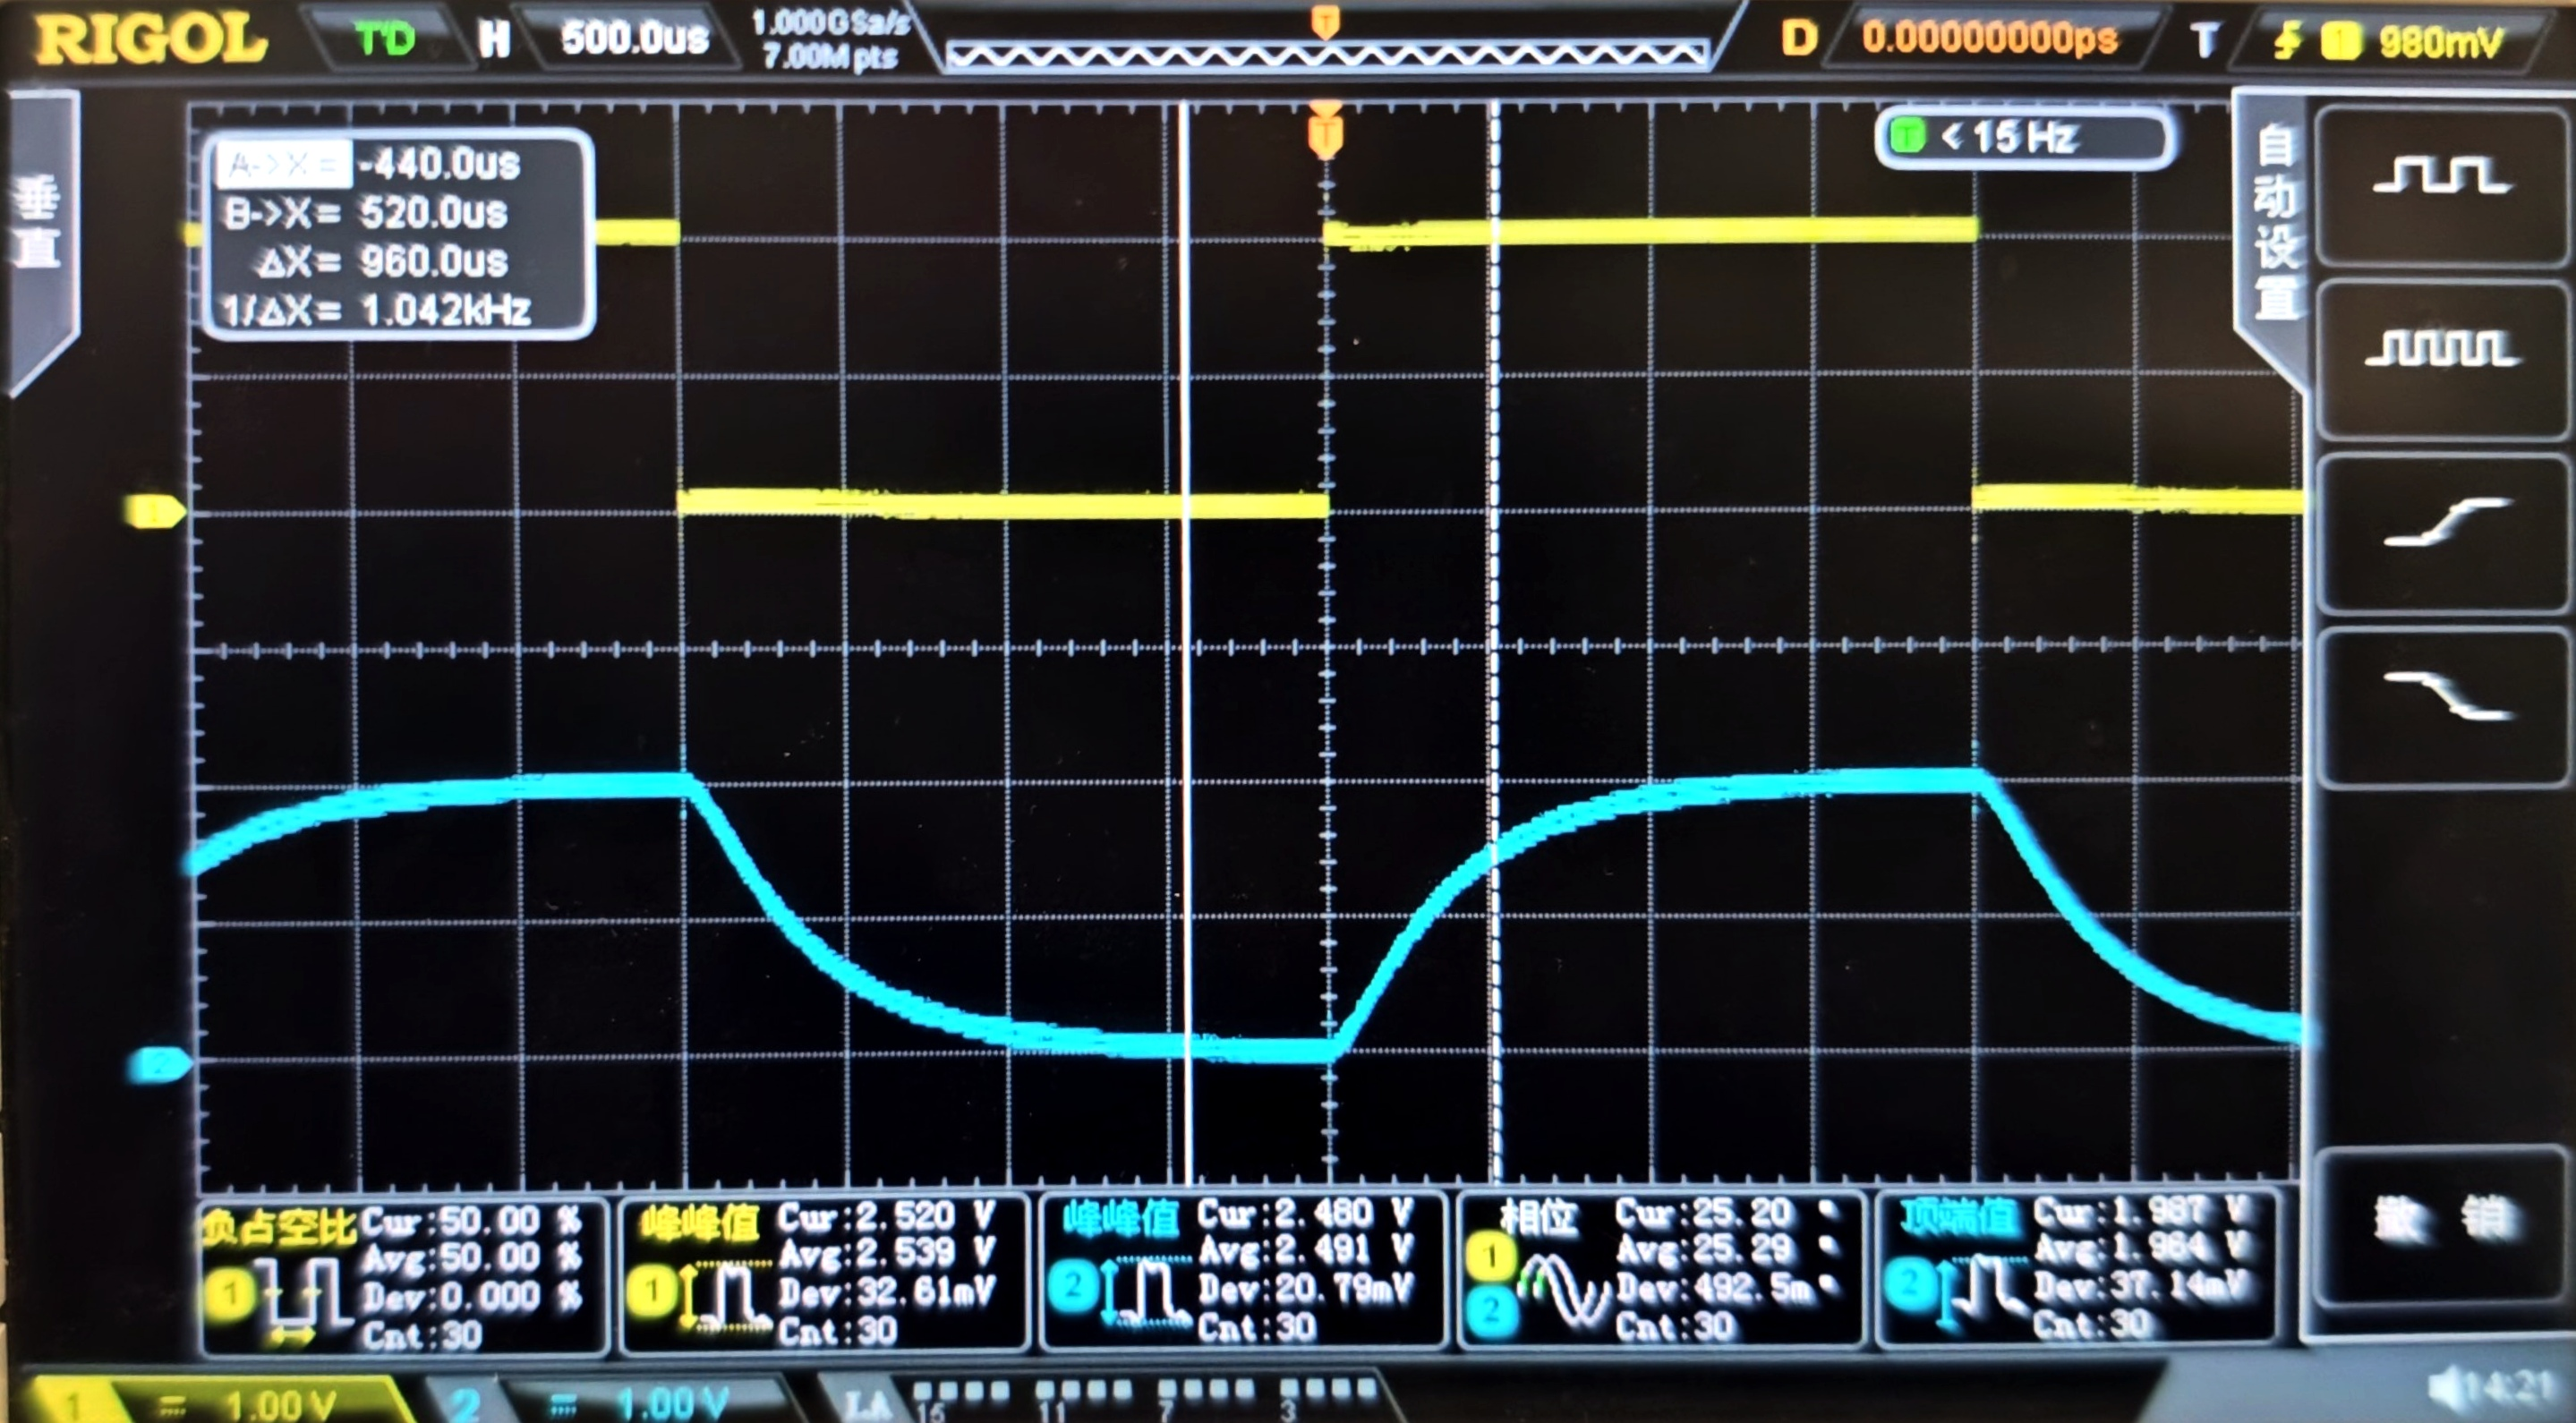
\includegraphics[width=\textwidth]{rlc_transient_R20k.jpg}
        \caption{强过阻尼 ($R=\SI{20}{\kilo\ohm}$)}
        \label{fig:rlc_trans_R20k}
    \end{subfigure}
    \caption{不同阻尼状态下的$u_C$暂态波形}
    \label{fig:rlc_transient_waveforms}
\end{figure}

\subsubsection{数据分析}
\begin{enumerate}
    \item \textbf{临界电阻理论值计算}
    
    根据RLC串联电路暂态理论，临界阻尼电阻 $R_{\text{cr}}$ 计算公式为：
    \[ R_{\text{cr}} = 2\sqrt{\frac{L}{C}} \]
    代入实验参数 $L=\SI{0.1}{\henry}$，$C=\SI{0.2}{\micro\farad}$，计算得：
    \[ R_{\text{cr}} = 2\sqrt{\frac{0.1}{0.2 \times 10^{-6}}} = 2\sqrt{500000} \approx \SI{1414}{\ohm} \]

    \item \textbf{临界电阻测量与误差分析}
    
    实验中调节电阻箱，观测到波形处于临界阻尼状态（刚好无过冲且衰减最快）时，记录电阻箱阻值为 $R_{\text{meas}} = \SI{800}{\ohm}$。
    
    与理论值相比，相对误差为：
    \[ \delta = \left| \frac{R_{\text{meas}} - R_{\text{cr}}}{R_{\text{cr}}} \right| \times 100\% = \left| \frac{800 - 1414}{1414} \right| \times 100\% \approx 43.4\% \]
    
    \textbf{误差来源分析}：
    \begin{itemize}
        \item \textbf{电路固有电阻未计入}：实验记录的 $800\,\Omega$ 仅为电阻箱阻值。实际电路总电阻还应包含电感线圈的直流内阻 $R_L$（通常在 $100\sim 300\,\Omega$ 之间）以及函数发生器的输出阻抗（通常为 $50\,\Omega$）。若计入这些电阻，实际总电阻将更接近理论值。
        \item \textbf{临界状态判读的主观性}：在示波器上通过肉眼观察波形来判断“刚好无振荡”的临界点存在较大主观误差，往往难以精确区分微弱的欠阻尼状态与临界状态。
        \item \textbf{元件参数偏差}：电感 $L$ 和电容 $C$ 的实际值可能与标称值存在偏差，导致理论计算基准偏移。
    \end{itemize}

    \item \textbf{阻尼状态判定}
    \begin{itemize}
        \item 当 $R = \SI{0}{\ohm}$ 时，$R < R_{\text{cr}}$，理论上电路应处于欠阻尼状态。实验波形（图\ref{fig:rlc_trans_R0}）显示明显的振荡衰减特征，与理论一致。
        \item 当 $R = \SI{2}{\kilo\ohm}$ 时，$R > R_{\text{cr}}$，理论上电路应处于过阻尼状态。实验波形（图\ref{fig:rlc_trans_R2k}）显示电压单调趋近稳态值，无振荡现象，验证了过阻尼特性。
        \item 当 $R = \SI{20}{\kilo\ohm}$ 时，$R \gg R_{\text{cr}}$，电路处于强过阻尼状态。实验波形（图\ref{fig:rlc_trans_R20k}）显示过渡过程显著延长，衰减极为缓慢。
    \end{itemize}
\end{enumerate}

\subsubsection{实验总结}
\begin{enumerate}
    \item \textbf{阻尼规律验证}：实验清晰地展示了电阻对RLC串联电路暂态过程的影响。随着电阻 $R$ 的增大，电路从欠阻尼振荡逐渐过渡到过阻尼非振荡状态，且过阻尼程度越深，系统响应速度越慢（时间常数 $\tau$ 增大）。
    
    \item \textbf{激励频率的选择}：为了完整观测暂态过程，方波激励的半周期应大于电路的暂态调节时间。实验中针对不同阻尼工况调整了方波频率（欠阻尼时较高，强过阻尼时较低），确保了波形的完整性与清晰度。
    
    \item \textbf{误差来源}：实验中观察到的波形与理论预测高度吻合。微小偏差可能来源于电感线圈的直流电阻（使得 $R=0$ 时实际阻尼系数不完全为0）、电容的漏电流以及示波器读数误差。
\end{enumerate}

\section{结论与心得体会}

\subsection{实验结论}
通过本次实验，我对RLC电路的稳态谐振特性与暂态响应规律有了深入的理解，主要结论如下：
\begin{enumerate}
    \item \textbf{串联谐振特性}：RLC串联电路在谐振时表现出纯阻性，阻抗最小，电流最大。实验验证了谐振频率 $f_0$ 由 $L, C$ 决定，且电路具有电压放大作用（$Q > 1$时，$u_L, u_C > u$）。通过频带宽度法和电压比法测得的品质因数 $Q$ 值吻合良好，验证了理论的正确性。
    \item \textbf{并联谐振特性}：RLC并联电路在谐振时表现出高阻抗特性，总电流最小，支路电流远大于总电流（电流放大）。实验测得并联电路的 $Q$ 值显著高于串联电路（约55 vs 12），说明减少回路中的损耗电阻能显著提高电路的选频性能。
    \item \textbf{暂态过程规律}：电路的暂态响应取决于阻尼系数。实验清晰观测到了欠阻尼（振荡衰减）、临界阻尼（最快无振荡衰减）和过阻尼（缓慢非振荡衰减）三种状态，验证了电阻 $R$ 对电路动态特性的调控作用。
\end{enumerate}

\subsection{问题讨论}
在实验过程中，遇到了一些值得探讨的问题：
\begin{enumerate}
    \item \textbf{临界电阻测量值的偏差}：在暂态实验中，测得的临界电阻（$800\,\Omega$）远小于理论计算值（$1414\,\Omega$）。经过分析，这主要是因为理论计算未包含电感线圈的直流内阻（通常可达几百欧姆）以及信号源的输出阻抗（$50\,\Omega$）。实际电路的总电阻是电阻箱读数与这些固有电阻之和，因此电阻箱只需调到较小值即可达到临界阻尼条件。这一现象提醒我们在进行电路设计和分析时，不能忽视非理想元件的寄生参数。
    \item \textbf{谐振点的精确判断}：在测量频率特性时，仅凭示波器观察电压最大值或相位差为零来确定谐振频率存在一定的主观误差。采用李萨如图形法辅助判断相位差为零，或者使用数字万用表监测电压极值，可以提高测量的准确度。
\end{enumerate}

\subsection{心得体会}
本次实验不仅加深了我对电路理论的认识，也锻炼了我的实验操作技能：
\begin{enumerate}
    \item \textbf{理论与实践的结合}：书本上的公式（如 $Q$ 值定义、阻尼条件）在实验波形中得到了直观的验证，让我深刻体会到物理模型与实际电路之间的联系与差异（如寄生参数的影响）。
    \item \textbf{仪器使用的熟练度}：通过实验，我更加熟练地掌握了数字存储示波器的使用，特别是利用光标测量时间差计算相位、利用存储功能捕捉暂态波形等技巧，这对今后的科研工作大有裨益。
    \item \textbf{严谨的科学态度}：面对实验数据与理论值的偏差（如临界电阻），不能简单地归结为“误差”，而应深入分析电路结构寻找原因。这种探究过程比单纯验证理论更有价值。
\end{enumerate}
\section{原始图片}
\begin{figure}[htbp]
    \centering
        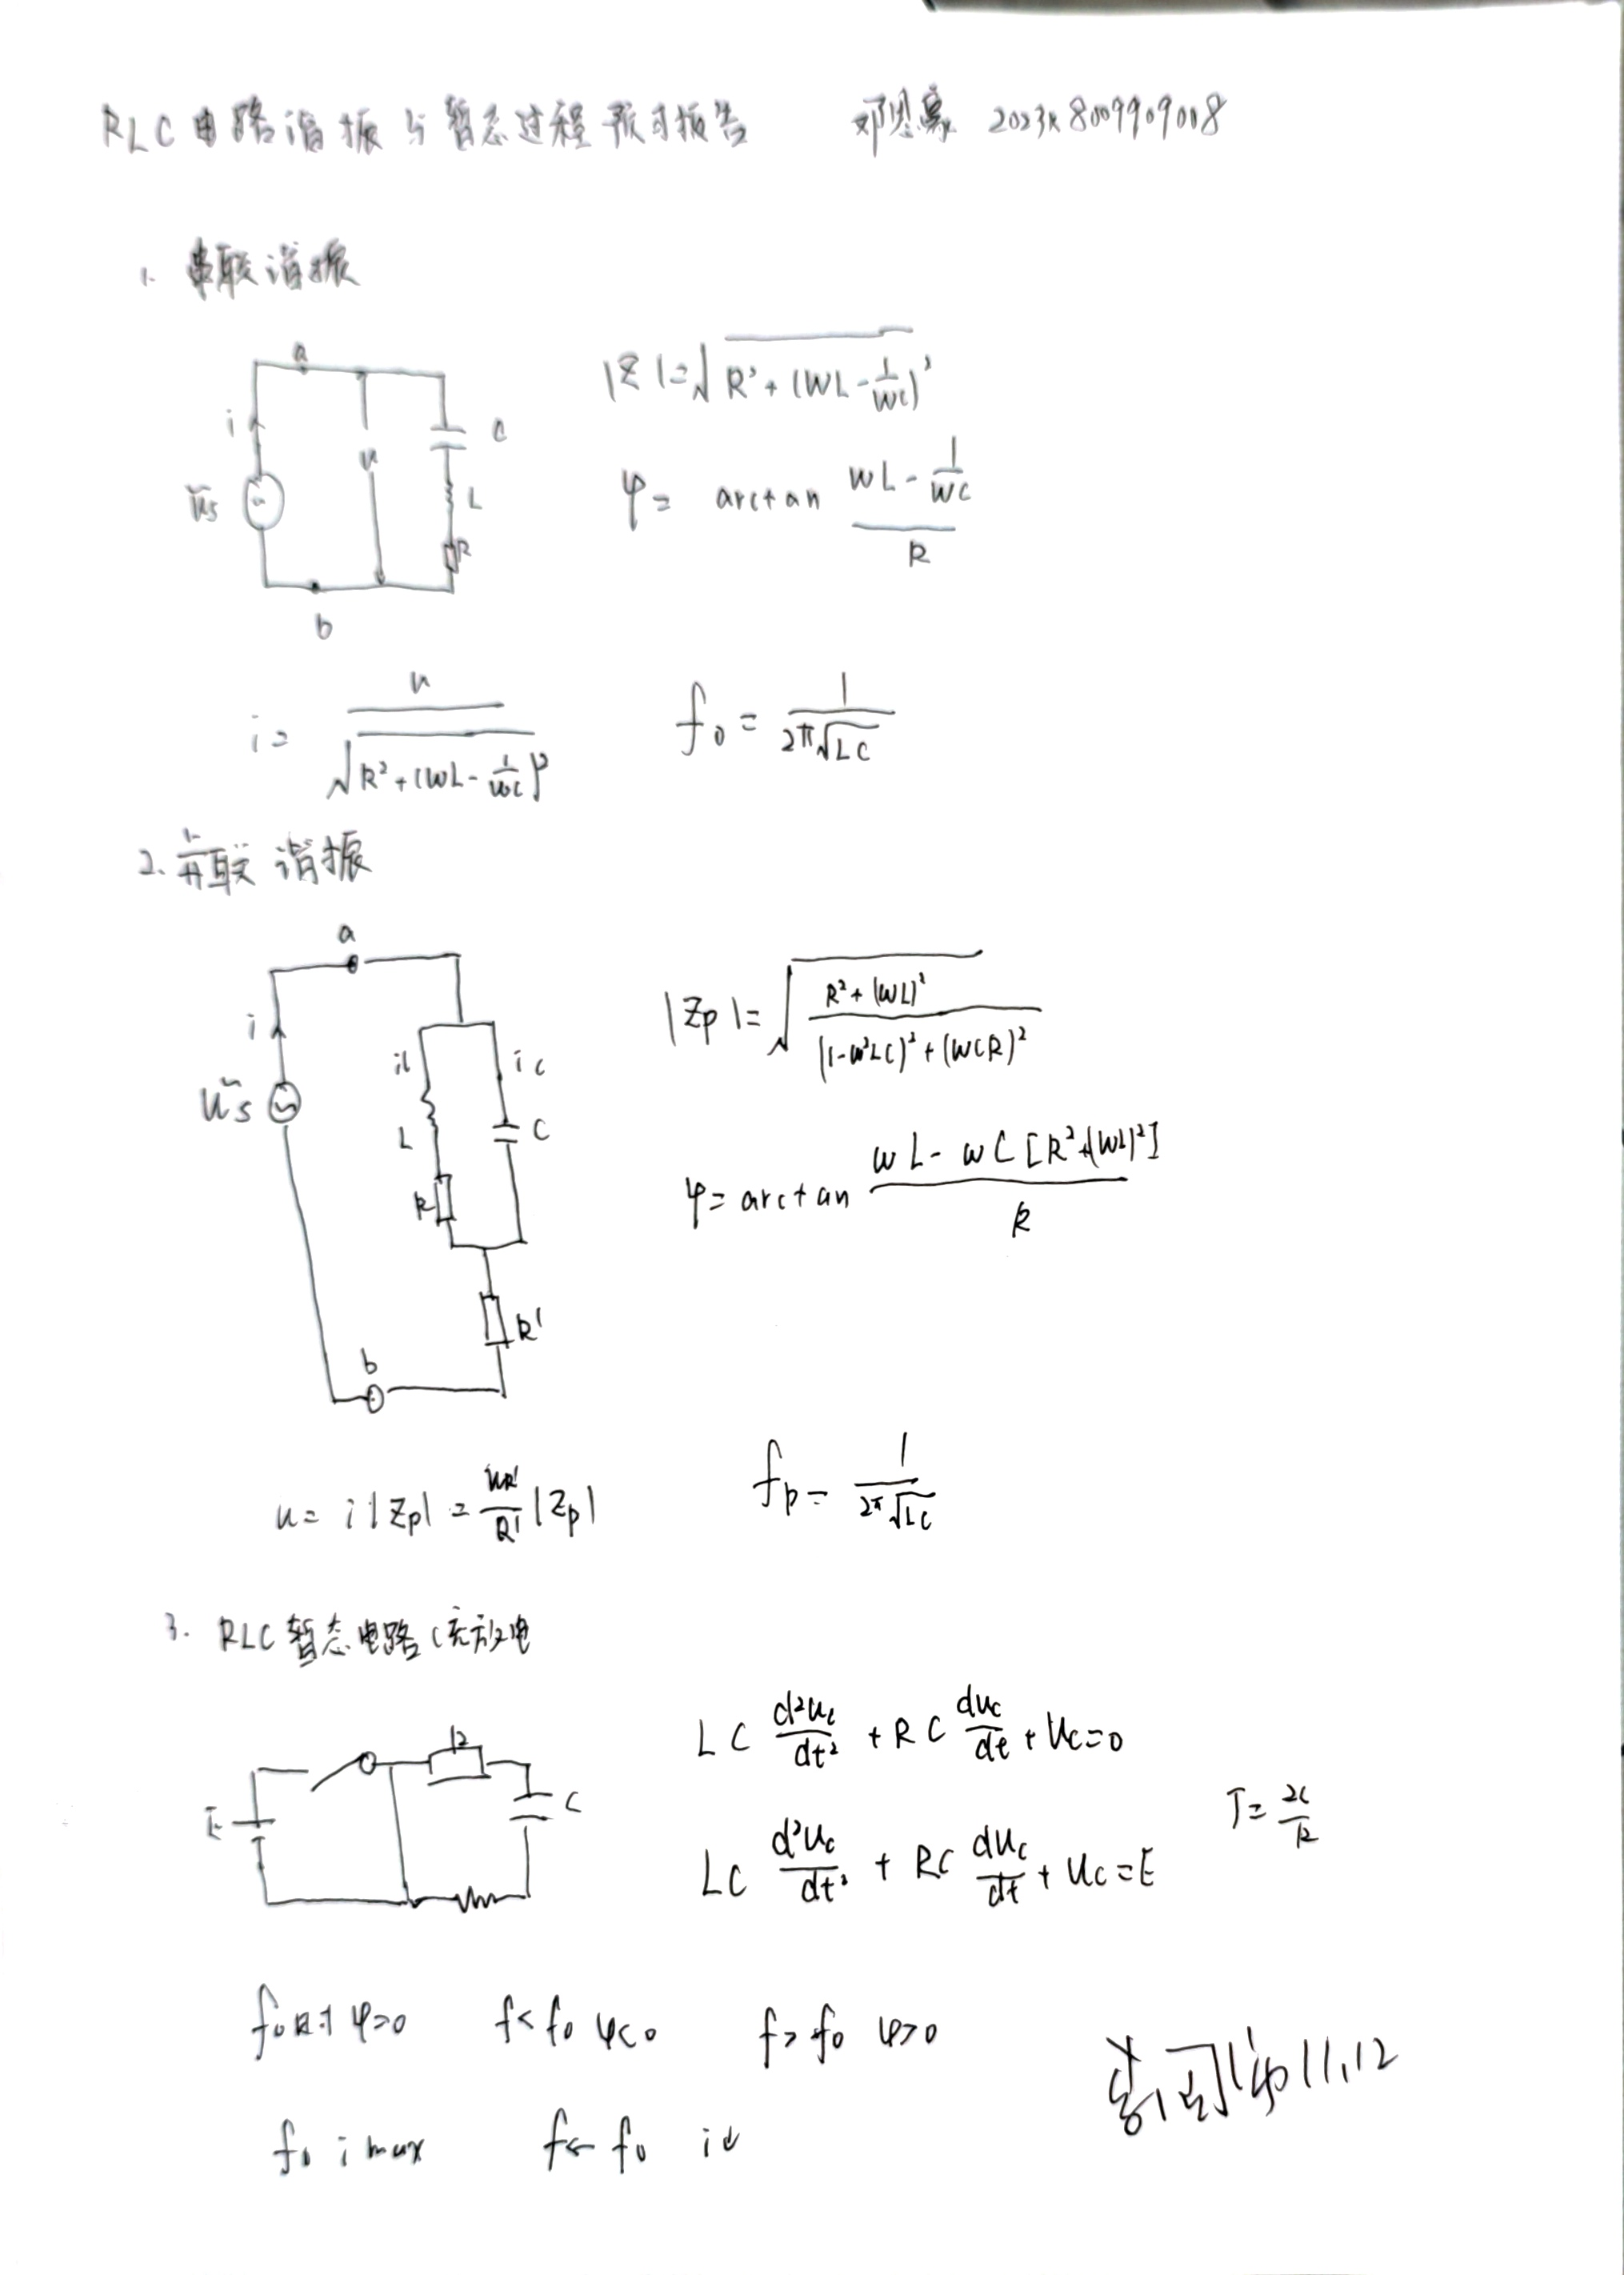
\includegraphics[width=\textwidth]{IMG_20251229_201327.jpg}
\end{figure}
\begin{figure}[htbp]
    \centering
        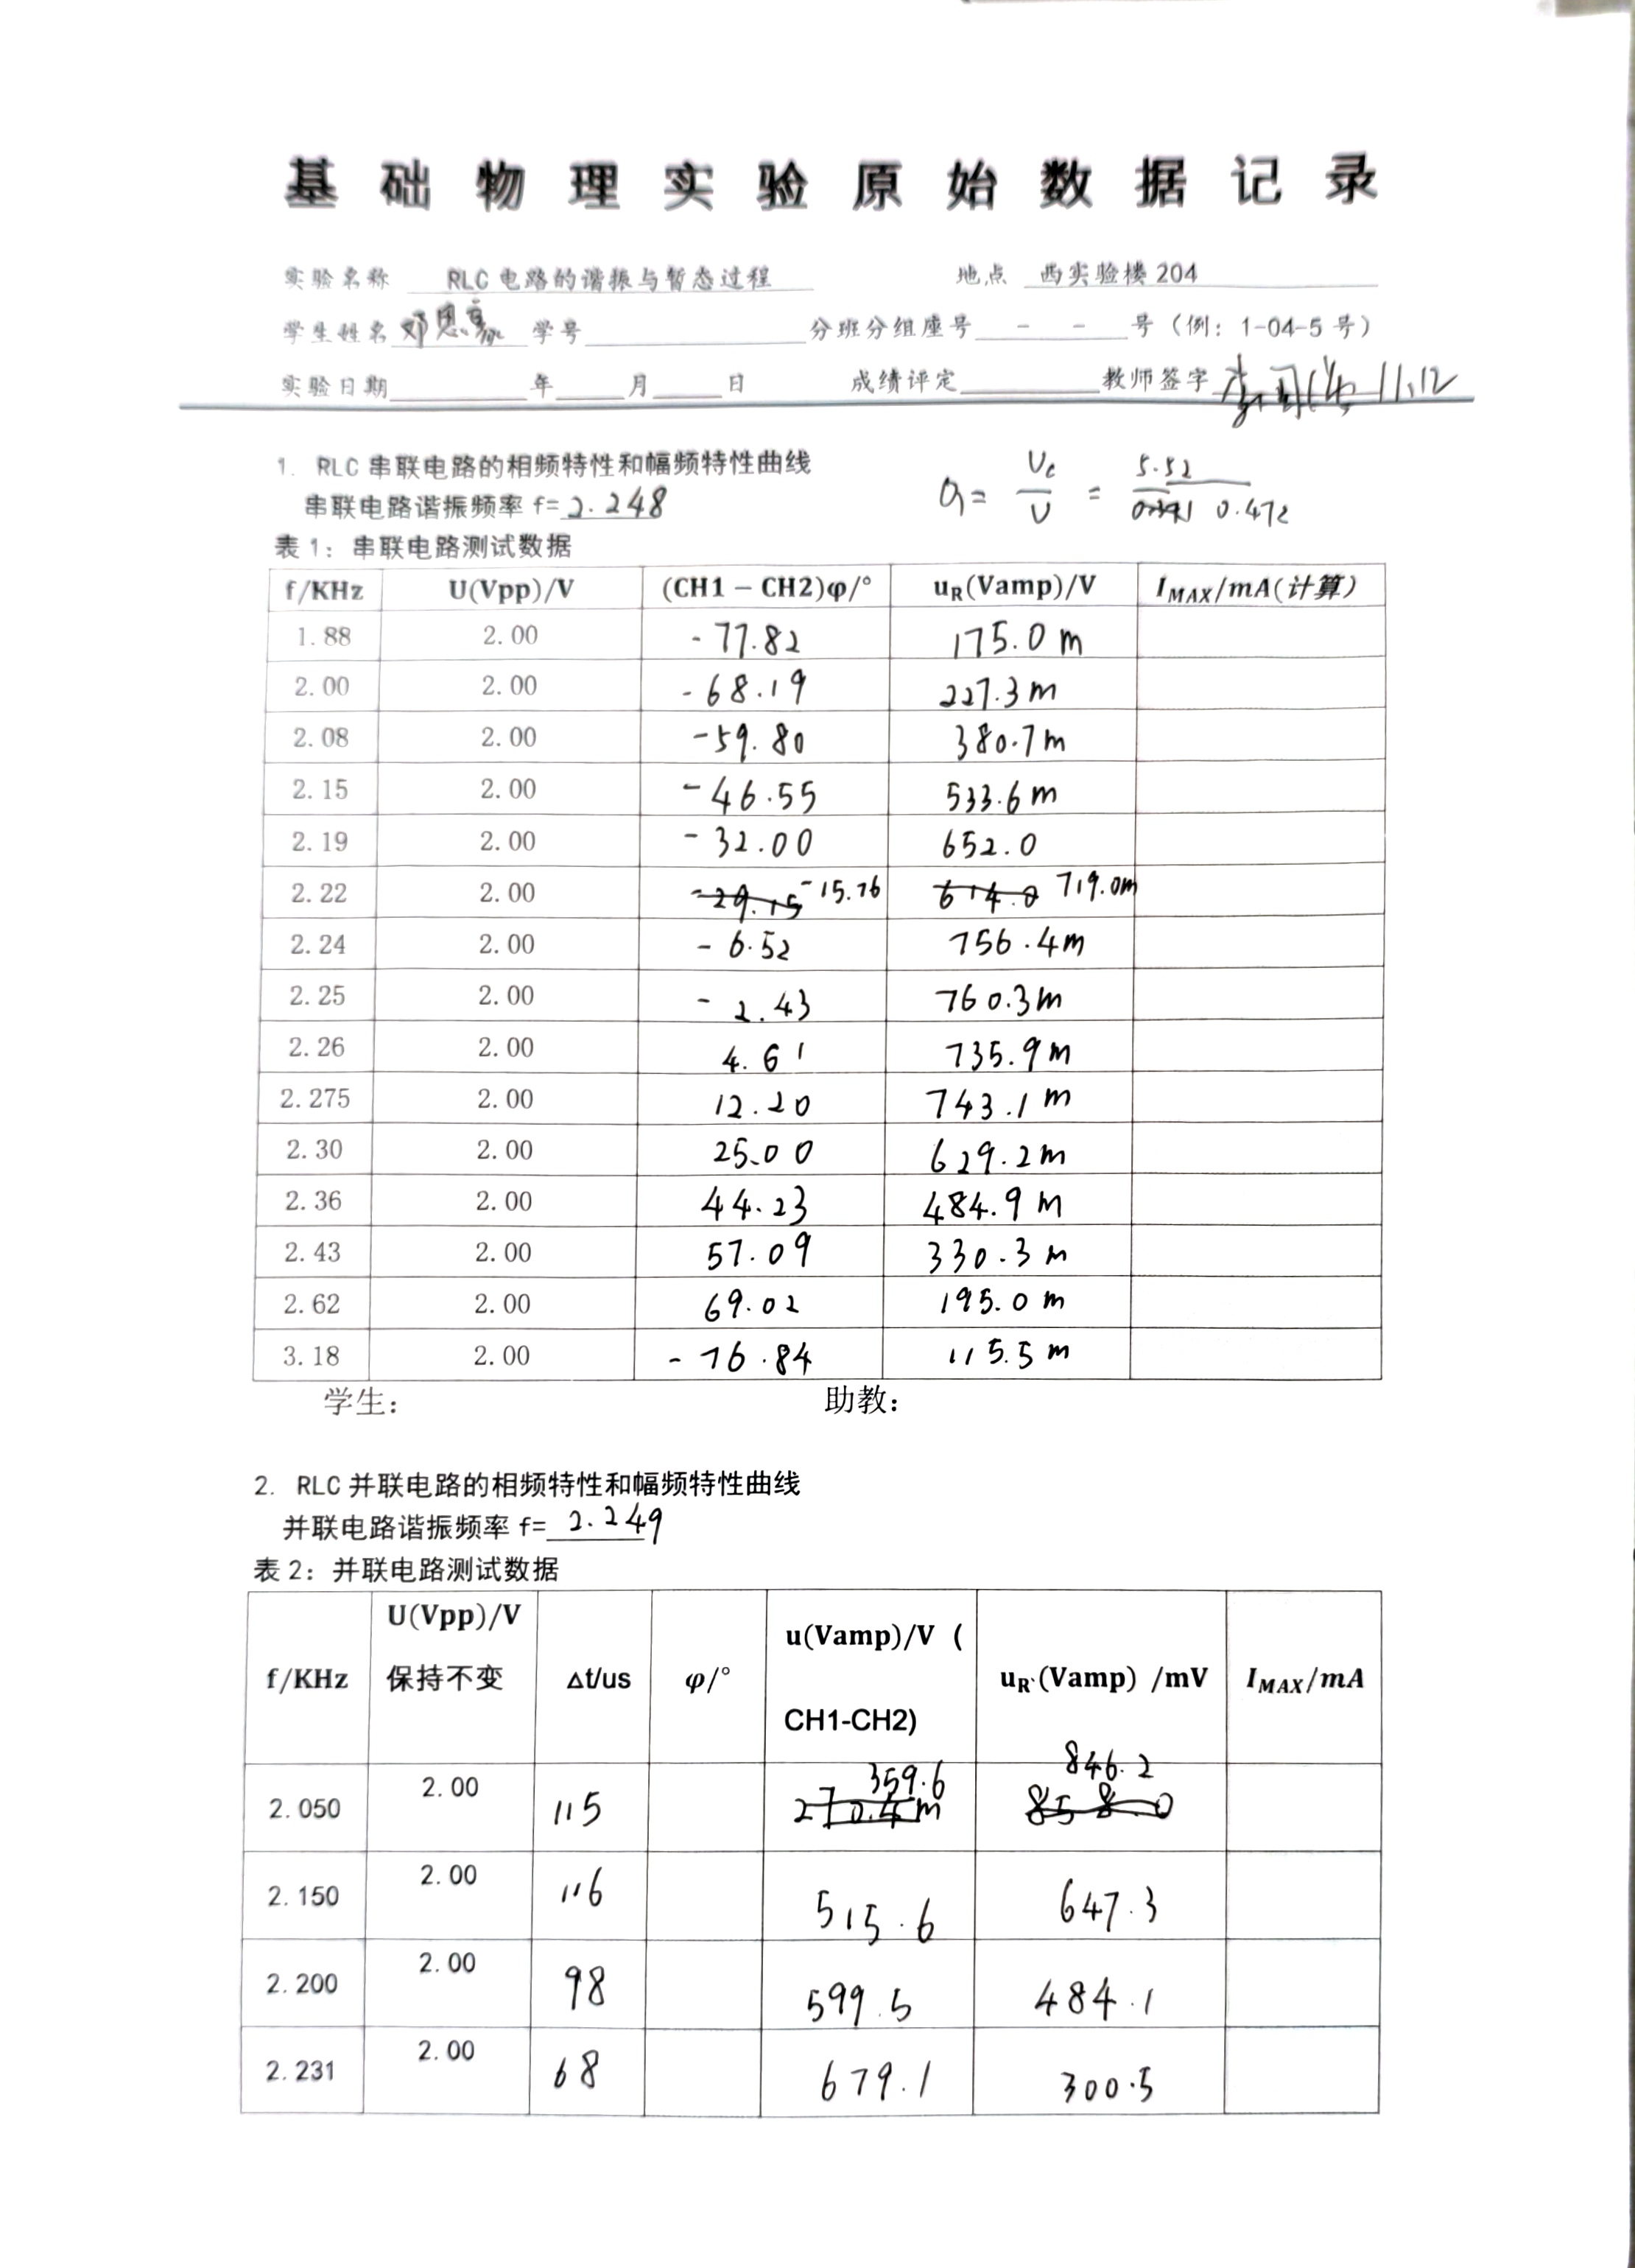
\includegraphics[width=\textwidth]{IMG_20251229_201331.jpg}
\end{figure}
\begin{figure}[htbp]
    \centering
        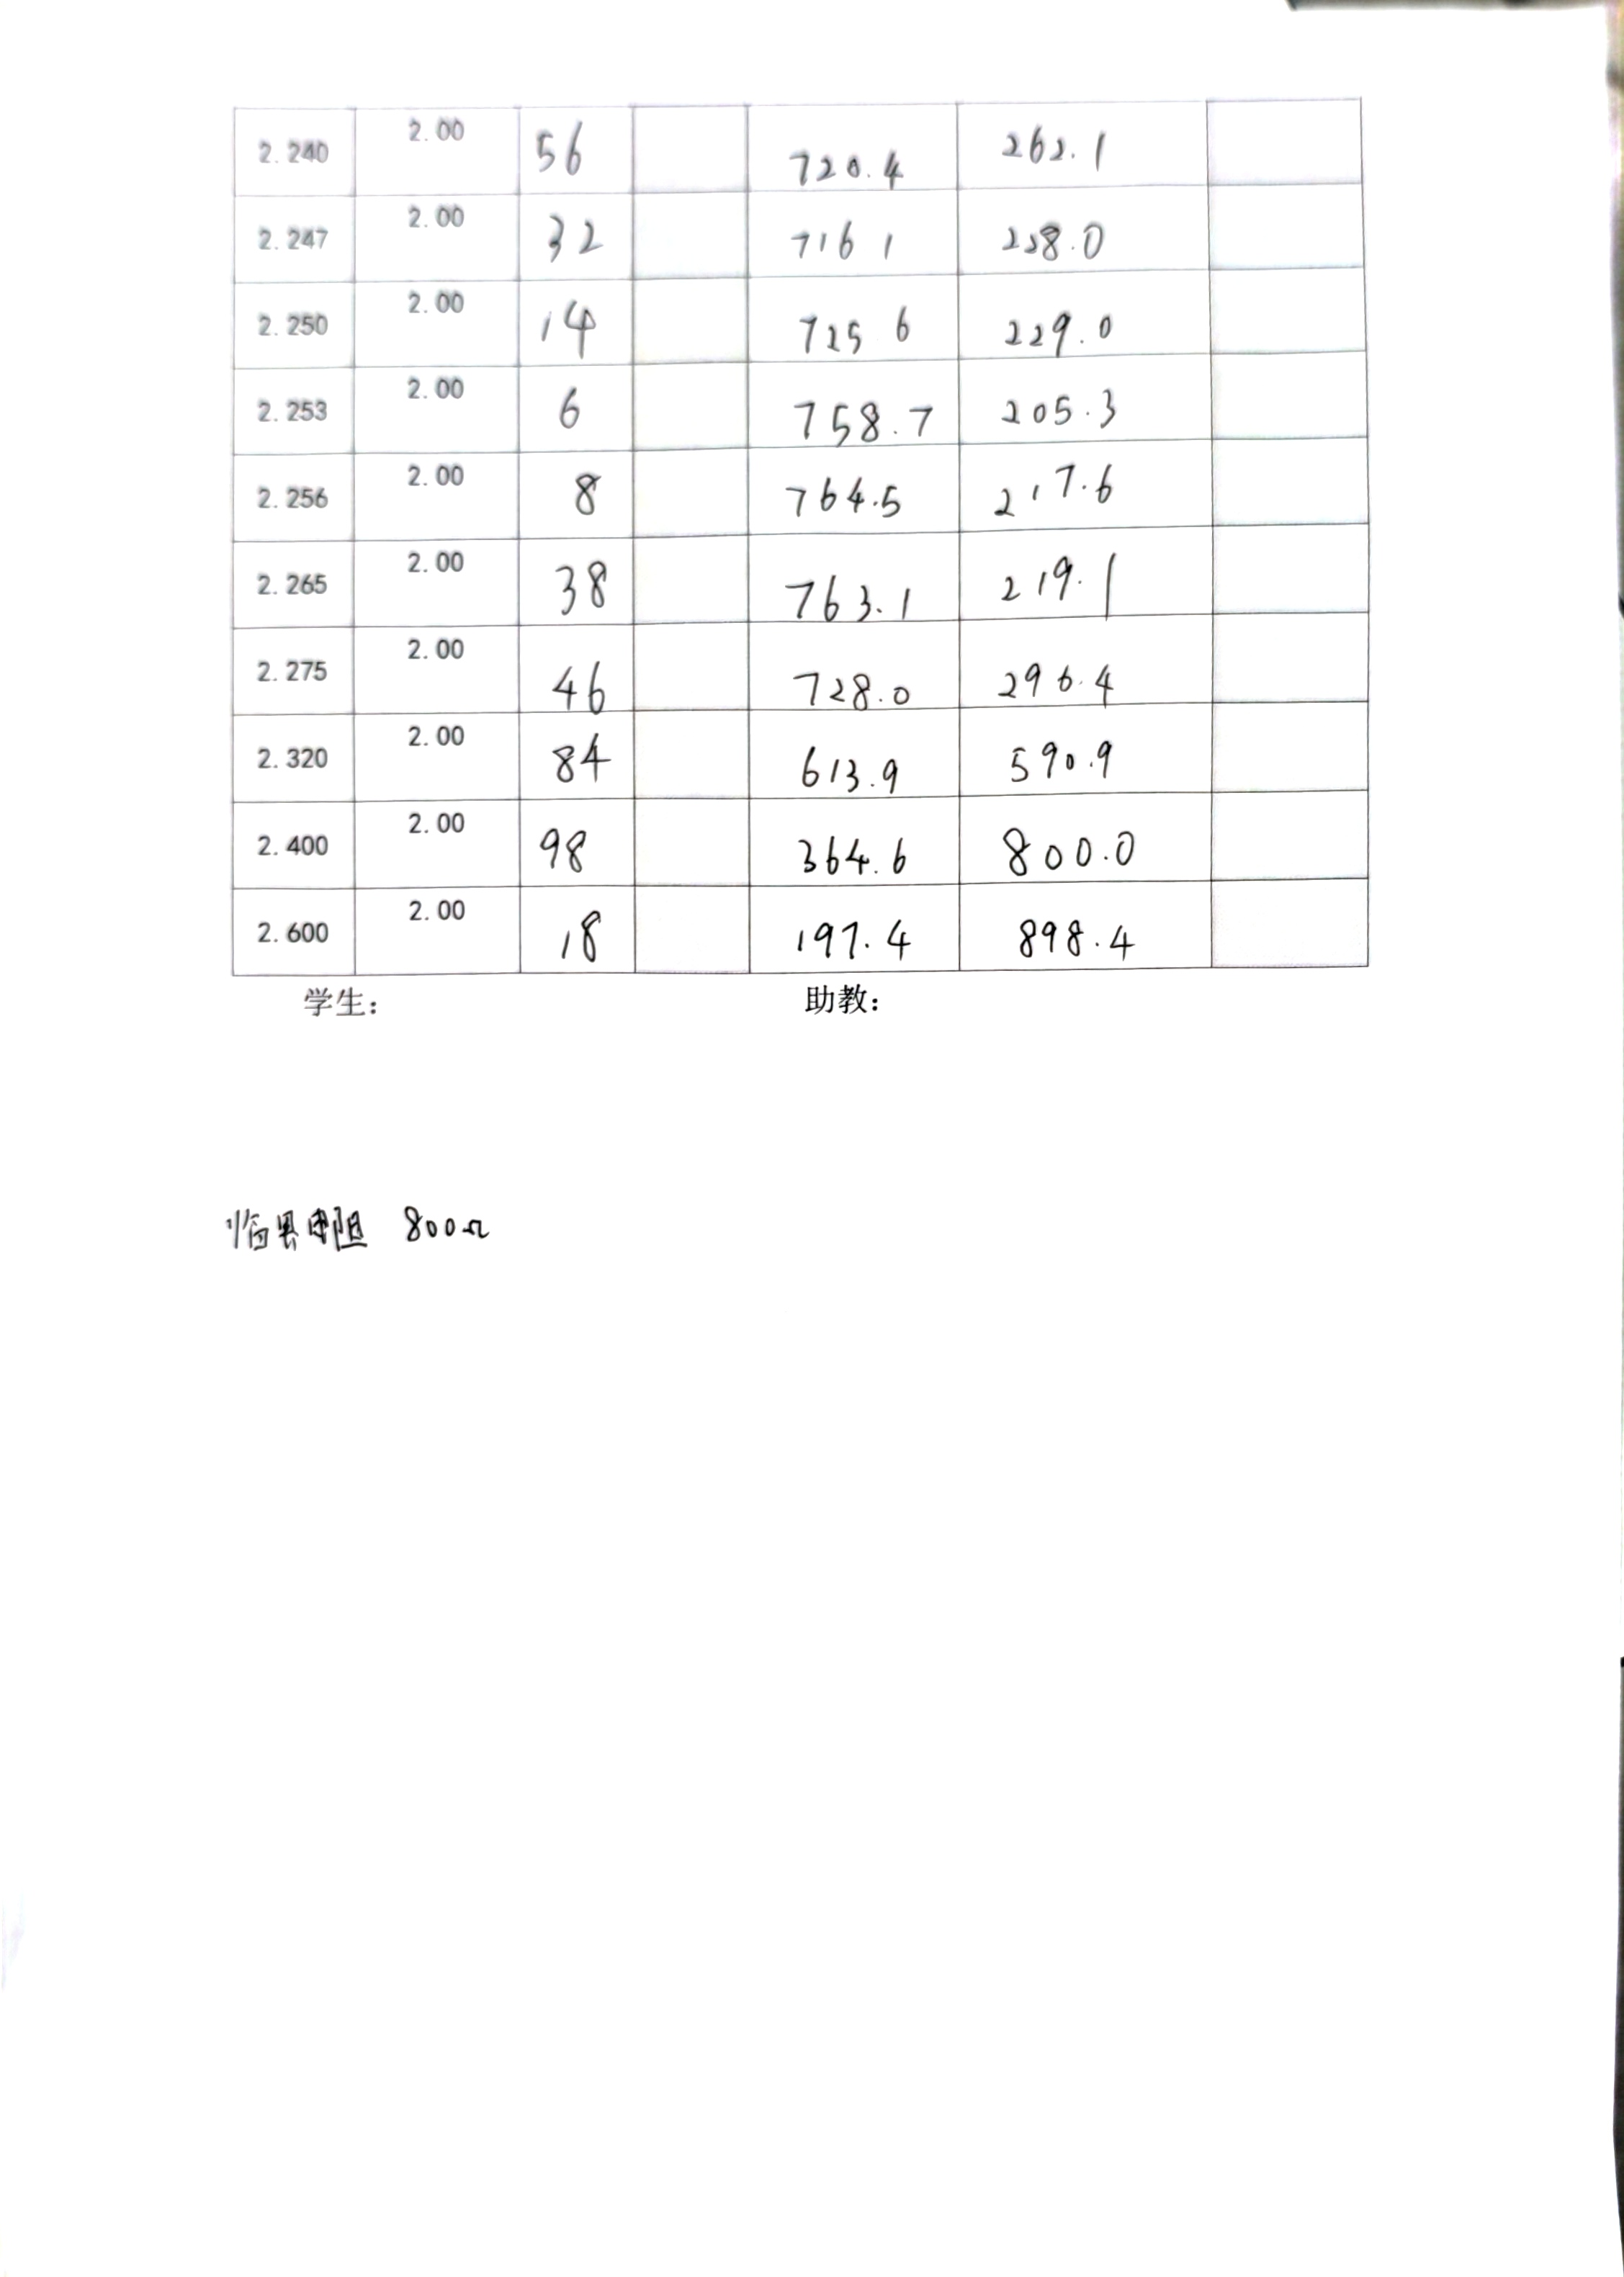
\includegraphics[width=\textwidth]{IMG_20251229_201337.jpg}
\end{figure}
 
\end{document}